%=======================================================================
%  SNAPSHOT 2026-09-25, before demographics were split out of the paper.
%  This is the full version (exposure + siting + equity), kept as the seed of the
%  companion paper on siting and demographics. trames.tex is the surveillance-over-
%  time paper. Not built by default; tectonic trames-with-demographics-2026-09-25.tex works.
%=======================================================================
%  The Cost of Not Being Seen
%  Automated licence-plate reader exposure on American commutes,
%  and the price of avoiding it.
%
%  Build:  tectonic trames.tex
%=======================================================================
\documentclass[11pt,twoside]{article}

\usepackage[T1]{fontenc}
\usepackage[utf8]{inputenc}
\usepackage{lmodern}
\usepackage[margin=1in]{geometry}
\usepackage{graphicx}
\usepackage{booktabs}
\usepackage{amsmath,amssymb}
\usepackage{siunitx}
\usepackage{microtype}
\usepackage{caption}
\usepackage{subcaption}
\usepackage[table]{xcolor}
\usepackage{listings}
\usepackage{enumitem}
\usepackage{authblk}
\usepackage[numbers,sort&compress]{natbib}
\usepackage{xurl}
\usepackage[hidelinks,breaklinks]{hyperref}
\usepackage[capitalise,noabbrev]{cleveref}

\sisetup{group-separator={,},group-minimum-digits=4,group-digits=integer,detect-weight=true}
\captionsetup{font=small,labelfont=bf,width=.95\linewidth}
\captionsetup[sub]{font=small}
\setlist{itemsep=2pt,parsep=0pt,topsep=3pt}
% Let floats sit nearer their first mention: more of them per page, and float pages sooner.
\renewcommand{\topfraction}{0.85}\renewcommand{\bottomfraction}{0.6}
\renewcommand{\textfraction}{0.12}\renewcommand{\floatpagefraction}{0.75}
\setcounter{topnumber}{3}\setcounter{bottomnumber}{2}\setcounter{totalnumber}{4}
% Let a short page end short rather than stretching the space between paragraphs.
\raggedbottom

\definecolor{codebg}{HTML}{F6F6F6}
\lstset{
  basicstyle=\ttfamily\footnotesize,
  backgroundcolor=\color{codebg},
  frame=single, rulecolor=\color{gray!40},
  breaklines=true, showstringspaces=false,
  columns=fullflexible, xleftmargin=0pt, framexleftmargin=3pt,
}

% xspace must be loaded before the macro that uses it is expanded.
\usepackage{xspace}
\usepackage[super]{nth}
\newcommand{\alpr}{ALPR\xspace}
% OSM keys set in \texttt cannot hyphenate; let TeX stretch a line rather than overrun it.
\setlength{\emergencystretch}{2em}

\title{\bfseries The Cost of Not Being Seen:\\[2pt]
\large Automated Licence-Plate Reader Exposure on American Commutes\\
and the Price of Avoiding It}

% For submission: author names, affiliations and ORCIDs here; and, as the journal requires,
% statements on funding, competing interests, and whether institutional ethics review applied.
\author[ ]{TRAMES Project}
\affil[ ]{\small\texttt{kara@soulstone.org}}
\date{\today}

\begin{document}
\maketitle

% Long-form abstract (the earlier version, about 590 words), kept for a web or preprint page:
% Automated licence-plate readers (\alpr) have moved from tollbooths to residential
% intersections, and a single vendor---Flock Safety---now accounts for \SI{80.0}{\percent} of the
% \num{142991} installations mapped in North America. Public argument about this technology is
% conducted almost entirely in the abstract. We supply measurements instead: how much \alpr
% surveillance a typical American commuter drives through, what it would cost to refuse it,
% where the cameras stand relative to the people around them, and how those answers have changed
% as the map of cameras filled in.
%
% We build a continental routing engine that models \alpr fields of view as directional
% geometry---\SI{98.0}{\percent} of mapped cameras carry a bearing---and can be asked for a
% route that crosses none of them. We route \num{56131} real home--work commutes, drawn
% from Census LEHD LODES data in all fifty states and the District of Columbia and weighted to
% each state's commuters, twice each on an identical road network; and we compare every camera
% with a length-weighted sample of \num{11.2}~million points on roads of the same class in the
% same county.
%
% First, \SI{75.3}{\percent} of commutes pass at least one \alpr, a median of three and a
% \nth{99} percentile of thirty-four. Second, refusal is cheap: \SI{84.2}{\percent} of commutes
% can be routed to \emph{zero} \alpr exposure---the quarter that pass none, and four in five of the
% rest---and the avoiding route adds a median of \SI{1.62}{\minute}, an overhead of
% \SI{6.71}{\percent}, or \SI{3.14}{\minute} for commuters whose usual route passes a camera. Third, what commuters pass and where
% cameras stand answer the equity question differently. Gradients in commute exposure that
% appear robust nationally---origin tracts in the highest quartile of Hispanic population pass
% \num{1.46}$\times$ as many cameras as those in the lowest, and of Black population
% \num{1.39}$\times$---vanish when tracts are ranked within their own county (\num{1.01}$\times$
% and \num{1.06}$\times$). Siting does not. Compared with roads of the same class in the same
% county and density band, cameras stand \num{1.27}$\times$ as densely per kilometre of arterial
% in the most-Black tracts as in the least-Black, \num{1.59}$\times$ on residential streets and
% \num{1.87}$\times$ for police-operated cameras, a gradient that held across four maps while the
% map grew six-fold. Cameras follow traffic, but traffic does not explain the gradient: weighted
% by federal traffic counts, it is \num{1.20}$\times$ per vehicle-kilometre. Relative to other tracts, those neighbourhoods' cameras stand inside them
% rather than at their edges; it is wealthy neighbourhoods that concentrate their cameras at
% their edges, and the wealthiest towns that ring their limits most densely. The siting gradient
% is local, and most of the cameras a commute passes lie far from either end. Against the camera
% counts \num{1050} police departments publish, the map holds a median \SI{98}{\percent} of their
% cameras, with coverage unrelated to a city's Black share. By vendor, the other makers' cameras,
% more often on principal arterials and freeways, carry the steeper gradient in exposure
% (\num{1.57}$\times$ against \num{1.34}$\times$ for Flock nationally), but within counties Flock's
% cameras are sited as disproportionately as others' (\num{1.42}$\times$ against \num{1.44}$\times$).
%
% Finally, we reconstruct the camera map as it stood on five dates since January 2024 from
% OpenStreetMap's edit history---exactly, node for node---and route the same commutes against
% each. The map grew 128-fold, and measured exposure almost in proportion, from
% \SI{2.2}{\percent} of commuters passing a mapped reader to \SI{75.3}{\percent}; refusing them
% grew dearer, per camera as well as in total. The national exposure gradients moved with the
% map---the income contrast was \num{1.58}$\times$ in January 2025 and is \num{1.05}$\times$
% today---a warning to any study that reads equity from a crowdsourced map without asking when
% the map was drawn.
%
% All code, data acquisition, and analysis are reproducible from public sources.

\begin{abstract}
\noindent
Automated licence-plate readers (\alpr) have spread from tollbooths to residential streets;
one vendor, Flock Safety, holds \SI{80}{\percent} of the \num{142991} installations mapped in
North America. We measure what that means for an ordinary trip. A continental routing engine
models each camera's field of view and can find a route that crosses none. We route
\num{56131} home--work commutes from all fifty states and the District of Columbia, with and
without avoidance, and compare every camera with a sample of the roads it could have stood
on. \SI{75.3}{\percent} of commuters pass at least one reader, a median of three.
Refusal is cheap: \SI{84.2}{\percent} can reach work past none, and avoiding adds a median of
\SI{1.62}{\minute} (\SI{3.14}{\minute} for commuters with a camera to avoid). The two equity
questions have different answers. National gradients in commute exposure---\num{1.46}$\times$
by Hispanic and \num{1.39}$\times$ by Black share of the home tract---vanish within counties.
Siting does not: within the same county and density band, cameras stand \num{1.27}$\times$ as
densely per kilometre of arterial road in the most-Black tracts as in the least-Black,
police-operated cameras \num{1.87}$\times$ per kilometre of road, and \num{1.20}$\times$ per
vehicle-kilometre of counted traffic; relative to other tracts, they stand inside those
neighbourhoods rather than at their edges. Where police departments publish camera counts, the
map holds a median \SI{98}{\percent} of them. Rebuilt on five earlier dates from OpenStreetMap's
edit history, the map grew 128-fold from January 2024, and the national exposure gradients
moved with it: a warning to any equity study built on crowdsourced data.

\smallskip\noindent\textbf{Keywords:} automated licence-plate recognition; surveillance;
route choice; volunteered geographic information; OpenStreetMap; spatial equity.
\end{abstract}

\section{Introduction}
\label{sec:intro}

Automated licence-plate readers (\alpr) photograph every passing vehicle, resolve the plate,
and retain the read \citep{finklea2024}. Unlike a traffic camera they are not triggered by an offence, and unlike
a patrol officer they do not tire. Fixed, pole-mounted units have spread from limited-access
highways into residential neighbourhoods, arterial roads, and the entrances of private
subdivisions \citep{lum2019,stanley2022}.

The public debate about this expansion is conducted in the vocabulary of policy: retention
windows, warrant requirements, audit logs, data-sharing agreements. What that vocabulary
lacks is a measurement of the thing being regulated. How much of this does a person
actually drive through on an ordinary Tuesday? And if they would rather not, is declining
a practical option or a theoretical one?

This paper answers both, and does so by building the instrument the question implies. We
construct a routing engine that treats \alpr fields of view as first-class geometry and
can be asked for a route that avoids them. Running each sampled commute through it
twice---once normally, once avoiding---yields the exposure and the price of refusing it, for
the same trip, on the same network, at the same speeds.

The second quantity is where the paper earns its keep. A privacy protection that costs
four minutes is a feature. One that costs forty is available only to people with forty
minutes to spare, and a right that is priced is not evenly held. We therefore report the
cost of refusal across origin-tract income and racial composition---subject to the
substantial caveat developed in \Cref{sec:coverage} and quantified in
\Cref{sec:results:coverage}, which turns out to govern how the demographic results may be
read.

The equity question also has a second form. What a commuter passes is not where cameras are
placed, and the two can diverge: a camera ringing a neighbourhood may lie on no one's commute,
and one inside it may be passed only by the people who live there. We therefore also measure
siting directly, comparing every camera with the roads it could have stood on
(\Cref{sec:results:siting}). The two measures give different answers, and the difference is
itself a finding.

A third question follows from the data source. The cameras are mapped by volunteers, and
the map has grown 128-fold since January 2024. OpenStreetMap keeps every edit, so the
measurement can be repeated on the map as it stood on any past date; we repeat it on five.
How much surveillance a commuter drives through turns out to be, in large part, a question
of how much of it had been mapped---and that has consequences for every equity claim made
from such data.

\subsection{Contributions}

\begin{itemize}
  \item \textbf{A directional exposure model at continental scale.} Cameras are wedges,
    not circles. \SI{98.0}{\percent} of mapped North American \alpr installations carry a
    bearing tag, making this feasible nationally. Proximity-based counting inflates
    exposure by charging drivers for cameras aimed at the opposite carriageway; we do not
    do it.
  \item \textbf{Avoidance routing with no forked router.} \num{157084} camera cones, unioned
    into \num{135210} polygons, are compiled into a stock GraphHopper spatial index at import
    time, so an ordinary per-request custom model can reference them by name. No engine
    patches, no geometry in the request.
  \item \textbf{A commute-weighted rather than area-weighted sample.} \num{56131} real
    home--work pairs in all fifty states and the District of Columbia, drawn from LEHD
    LODES with probability proportional to worker count and weighted to each state's
    commuters.
  \item \textbf{A vendor-resolved account of exposure and siting.} Flock's cameras and
    other makers' are bought by the same kind of customer---police departments, where the
    operator is known---but stand differently: other makers' units are more often multi-headed
    and stand beside the busiest roads, and per unit deployed they generate 2.26 times as many
    camera encounters. In exposure, the national racial gradient is stronger for them than for the vendor
    that dominates both the network and the public argument about it; in siting, within
    counties, Flock's cameras are placed as disproportionately as anyone's.
  \item \textbf{A coverage-bias control that changes the conclusion.} We show that the
    national demographic gradients in commute exposure do not survive within-county ranking,
    quantify the \num{7.1}-fold per-capita spread in mapped density between states, in which
    mapping effort and deployment cannot be told apart, and argue this check should be
    mandatory for work of this kind.
  \item \textbf{Exposure distinguished from siting.} A case-control design compares every
    camera with a length-weighted sample of \num{11.2}~million points on roads of the same
    class, county by county, and on the federal-aid network with each road weighted by its
    counted traffic. It finds what the commute measure cannot: within a county, cameras stand
    \SIrange{27}{59}{\percent} more densely per kilometre in the most-Black tracts and
    \SI{20}{\percent} more densely per vehicle-kilometre, inside those neighbourhoods rather than
    at their edges, while wealthy neighbourhoods and towns concentrate
    theirs at their edges and limits. Within a county, what commuters pass is close to equal;
    where cameras stand is not.
  \item \textbf{An external check of crowdsourced coverage.} Against the counts \num{1050}
    police departments publish in Flock's transparency portals, the map holds a median
    \SI{98}{\percent} of their cameras, and how completely a city is mapped is unrelated to its
    Black share.
  \item \textbf{A thirty-three-month trend on a fixed sample.} The camera map, reconstructed
    exactly from OpenStreetMap's edit history on five dates since January 2024, with the
    same commutes routed against each: exposure rose almost in proportion to the map,
    refusal grew dearer per camera as well as in total, and the national equity gradients
    moved with the map while the within-county ones converged toward parity.
\end{itemize}

\section{Related work}
\label{sec:related}

This paper sits where four bodies of work meet: research on \alpr as a policing technology, on
where surveillance is sited and on whom it falls, on volunteered geographic data and its biases,
and a small practice of routing around surveillance. We take them in turn, with the literature
on spatial inference that shapes the design, and then state what is, to our knowledge, new here.

\paragraph{\alpr as a policing technology.} Criminological research on \alpr has mostly asked
whether it works. \citet{lum2011} tested \alpr-equipped patrols in crime hot spots with a
place-based randomized design across two jurisdictions, and \citet{lum2025} review the impact
studies since, asking whether the technology's cost-effectiveness can be established at all.
\citet{shjarback2025} evaluate the Atlantic City Police Department's installation of fixed
readers on all entrances and exits to the city, reporting reductions in shootings, motor-vehicle
theft and property crime but not in violent crime overall. Sociological and legal work asks what
the technology does to policing itself. \citet{brayne2017}'s fieldwork in the Los Angeles Police
Department shows plate readers lowering the threshold for inclusion in police data to people with
no police contact, and \citet{joh2016} and \citet{ferguson2017} describe the automated suspicion
and data-driven policing such systems enable. \citet{monahan2026} examines Flock's network as a
communicative infrastructure through which discriminatory policing crosses jurisdictions. The
legal status of the resulting location records is unsettled: in \emph{Carpenter v. United States}
the Supreme Court held that obtaining historical cell-site location records is a Fourth Amendment
search \citep{carpenter2018}, and
\citet{finklea2024} reviews the questions law-enforcement \alpr use raises. None of this work
measures how much \alpr surveillance an ordinary trip passes.

\paragraph{Where surveillance is sited, and on whom it falls.} A second literature asks who is
watched. The closest precedent for our siting analysis is \citet{keener2026}, who mapped the 614
Flock camera locations in Hampton Roads, Virginia, that a federal court unsealed, and found
majority-Black tracts carrying about four times the cameras of majority-white ones and
high-poverty tracts more than twice those of low-poverty ones. A Cybernews analysis reported by \citet{cybernews2026} correlates
some \num{131000} DeFlock-mapped Flock cameras with state and county demographics, finding more
cameras per resident where Black (at the state level) or Hispanic and Native American (at the
county level) population shares are higher, and where poverty is lower. Earlier work asks the
same question of other technologies and places. In Oakland, eight days of police \alpr data
showed scans concentrated in low-income, Black and Latino neighbourhoods \citep{maass2015}; in
New York, a crowdsourced survey of some \num{25500} cameras found facial-recognition-capable
cameras more concentrated where more residents are not white, in the Bronx, Brooklyn and
Queens \citep{amnesty2022}; in Chicago,
gunshot-detection sensors cover only the police districts with the largest Black and Latinx
populations \citep{macarthur2021}, and automated traffic cameras, though not sited
disproportionately near Black or Latino neighbourhoods, ticket drivers from them at about twice
the rate \citep{sutton2022,hopkins2022}. Behind these measurements sits a theoretical literature
on the racialization of surveillance \citep{browne2015,benjamin2019}. These studies measure
siting, scans or tickets within one city or region, or correlate counts across states and
counties; none compares where cameras stand with what people pass while travelling, and all but
\citet{keener2026} rest on data whose completeness is unmeasured.

\paragraph{Volunteered geographic data.} The camera map is volunteered geographic information
\citep{goodchild2007}, whose quality has been assessed against authoritative data since
OpenStreetMap's early years \citep{haklay2010} and whose completeness is known to vary with place
and development \citep{herfort2023}. For surveillance specifically, the Atlas of Surveillance
records which agencies use which technologies but not where devices stand \citep{atlas}; DeFlock
supplies the locations \citep{deflock}. Coverage bias is the central threat to every result built
on such data, and we know of no earlier measurement of it for \alpr; we compare the map with the
camera counts police departments publish in Flock's transparency portals
(\Cref{sec:results:siting}).

\paragraph{Exposure along the way, and the unit of analysis.} That exposure to a place-bound
feature depends on where people go and not only on where they live is the uncertain geographic
context problem \citep{kwan2012}; the contrast we draw between where cameras stand and what
commuters pass is an instance of it. Assigning tract attributes to the commuters who live there
invites the ecological fallacy \citep{robinson1950}, and results can depend on the areal unit
chosen \citep{openshaw1984}: we report the siting results at two units, and read every
demographic contrast as a statement about places, not persons. Within-county contrasts are
stratified in the manner of \citet{mantel1959}.

\paragraph{Routing around surveillance.} A route that avoids cameras is an older idea than
\alpr: in 2001 iSee computed ``paths of least surveillance'' around Manhattan's closed-circuit
cameras \citep{isee2001,schienke2002}, of which a civil-liberties survey had counted some
\num{2400} visible from the street \citep{nyclu2006}. Several services now route drivers around mapped
\alpr, some using each camera's field of view \citep{deflockmaps,flockhopper,banditkin,driversagainstflock},
and in network measurement \citet{edmundson2016} characterize, and try to avoid, Internet paths
through surveillance states. None publishes a measurement of how much surveillance ordinary
trips pass or what avoiding it costs; the routing engine here is the instrument for that
measurement, not its contribution.

\paragraph{What is new here.} To our knowledge this paper is the first to measure, nationally
and on real commute flows, how many \alpr fields of view commuters pass and what avoiding them
costs; the first to reconstruct the history of the crowdsourced \alpr map from OpenStreetMap's
edit record and show that equity estimates move with the map's completeness; and the first to
check that map's coverage against the camera counts police departments publish. Its siting analysis confirms,
nationally and with a design that compares cameras with roads of the same class in the same
county and with the traffic those roads carry, the disparity that \citet{keener2026} and the
Cybernews analysis \citep{cybernews2026} report---and qualifies it: within counties, the disparity lies in where cameras are placed rather than in how many a
commuter passes.

\section{System}
\label{sec:system}

\subsection{Why a fork, and of what}

The measurement needs a router that treats ``avoid these \num{135210} polygons'' as a
cost rather than a post-hoc filter, and the eventual application needs to be a real
navigation client rather than a research script.

\textbf{OsmAnd} \citep{osmand} is the base: a mature open-source Android navigation client
with first-class OpenStreetMap support, offline maps, and a documented online-routing
extension point. Its \emph{code} is GPLv3; its \emph{artwork} is CC-BY-NC-ND 4.0 and must
therefore be replaced rather than modified in a derivative.

\textbf{GraphHopper 11.0} \citep{graphhopper11} is the routing engine. Valhalla was
evaluated and rejected: its \texttt{exclude\_polygons} support has a record of routes passing
\emph{through} the excluded region, one a genuine defect fixed only in December 2025
\citep{valhalla5069} and another report still open \citep{valhalla4659}---and a route through
an excluded region is precisely the error everything here depends on not making.

One architectural property made the rest tractable. OsmAnd's online routing engines return
\emph{geometry only}; turn instructions are re-derived client-side from offline map data.
A custom online router therefore never has to synthesise navigation instructions.

\subsection{The keystone: import-time custom areas}

GraphHopper resolves \texttt{custom\_areas.directory} into a spatial index \emph{at graph
import time}. We verified empirically---the documentation is ambiguous---that an area
registered this way can be referenced by name from a \emph{per-request} custom model:

\begin{lstlisting}[language=]
{ "priority": [ { "if": "in_alpr", "multiply_by": 0.01 } ] }
\end{lstlisting}

\noindent
This is what makes the design possible without forking the engine; shipping \num{135210}
polygons in every routing request is not viable. The cost is that regenerating cones
requires a full re-import (\SI{82}{\minute} to \SI{113}{\minute} for North America, by load).

Two further configuration decisions are load-bearing:

\begin{itemize}
  \item \textbf{Contraction Hierarchies are disabled.} CH \citep{geisberger2008} bakes edge
    weights into the prepared graph, which is incompatible with a per-request avoidance
    strength. Landmarks (LM, the ALT algorithm of \citet{goldberg2005}) are used instead.
  \item \textbf{The \texttt{car\_alpr} profile shares \texttt{car}'s LM preparation.} This
    halves preparation time and is valid \emph{only} because avoidance multiplies priority
    strictly downward, so the borrowing profile's edge weights never fall below the preparation
    profile's: the landmark distances remain lower bounds, the condition LM correctness
    requires.
\end{itemize}

\subsection{Deployment posture}

The routing server binds to localhost. It has no authentication and no rate limiting and
is not internet-facing. Any public deployment must sit behind a reverse proxy supplying
both.

\section{Data}
\label{sec:data}

All sources are public and key-free.

\subsection{ALPR installations}
\label{sec:data:alpr}

Source: OpenStreetMap \citep{osm}, queried through the Overpass API \citep{olbricht2015} for nodes tagged
\texttt{man\_made=\allowbreak surveillance} with \texttt{surveillance:\allowbreak type=ALPR},
matched case-insensitively (19 readers are tagged \texttt{alpr})---the corpus surfaced by the
DeFlock project, taken from the upstream rather than a mirror. Retrieved in five regional
queries (continental US, Alaska, Hawaii, Canada, Mexico) and deduplicated by OSM node id.
The results in this paper rest on the snapshot of \textbf{2026-09-22: \num{142991} unique
camera nodes}, \num{142257} of them in the 50 states and the District of Columbia
(\Cref{fig:map}); the rest fall in the parts of Canada and Mexico the regional queries
cover. A first snapshot, taken 2026-07-24, held \num{120838} (\num{120272} in the states),
and \Cref{sec:data:history} reconstructs five earlier dates.

A fetch that fails over between Overpass mirrors has to check the mirror's database
date. On the first attempt at the September snapshot one regional query fell through to
a mirror whose database was dated 2026-05-06; that box overlaps the southern United
States, regions were merged last-wins, and roughly \num{13600} cameras across Texas,
Arizona and Florida silently reverted to four-month-old tags while some \num{400} nodes
deleted since May returned as ghosts. Nothing failed. The fetch now rejects any answer
older than 48 hours and merges overlapping regions newest-database-first; every tile of
the snapshot used here falls within a 14-minute window.

\begin{table}[tbp]
\centering
\small
\caption{Directional and vendor tagging across the two 2026 snapshots. The direction-key rows
overlap (392 and 415 nodes carry both keys). Vendors are matched as case-insensitive
substrings of the first of the four vendor keys present, in both columns.}
\label{tab:tags}
\begin{tabular}{lrrrr}
\toprule
& \multicolumn{2}{c}{2026-07-24} & \multicolumn{2}{c}{2026-09-22} \\
\cmidrule(lr){2-3}\cmidrule(lr){4-5}
Property & Count & Share & Count & Share \\
\midrule
Camera nodes                        & \num{120838} &                     & \num{142991} & \\
Any direction tag                   & \num{119249} & \SI{98.7}{\percent} & \num{140112} & \SI{98.0}{\percent} \\
\quad via \texttt{direction}        & \num{117356} & \SI{97.1}{\percent} & \num{138216} & \SI{96.7}{\percent} \\
\quad via \texttt{camera:direction} & \num{2285}   & \SI{1.9}{\percent}  & \num{2311}   & \SI{1.6}{\percent} \\
Multi-head (\texttt{;}-separated)   & \num{7014}   & \SI{5.8}{\percent}  & \num{9150}   & \SI{6.4}{\percent} \\
Arc-range form (\texttt{199-269})   & \num{4806}\,tokens & ---           & \num{4632}\,tokens & --- \\
\texttt{operator} tagged            & \num{22354}  & \SI{18.5}{\percent} & \num{23872}  & \SI{16.7}{\percent} \\
\midrule
Flock Safety                        & \num{99650}  & \SI{82.5}{\percent} & \num{114360} & \SI{80.0}{\percent} \\
Motorola Solutions                  & \num{5993}   & \SI{5.0}{\percent}  & \num{7411}   & \SI{5.2}{\percent} \\
Genetec                             & \num{2876}   & \SI{2.4}{\percent}  & \num{3721}   & \SI{2.6}{\percent} \\
Leonardo                            & \num{1020}   & \SI{0.8}{\percent}  & \num{1215}   & \SI{0.8}{\percent} \\
Axis Communications                 & \num{1052}   & \SI{0.9}{\percent}  & \num{3327}   & \SI{2.3}{\percent} \\
No vendor tag                       & \num{5811}   & \SI{4.8}{\percent}  & \num{6850}   & \SI{4.8}{\percent} \\
\bottomrule
\end{tabular}
\end{table}

Three tagging realities shaped the parser, each contradicting a plausible assumption:

\begin{enumerate}
  \item \textbf{\texttt{direction}, not \texttt{camera:direction}.} The OSM wiki documents
    \texttt{camera:direction} for surveillance nodes \citep{osmwikisurveillance}. Mappers overwhelmingly use plain
    \texttt{direction}, by a factor of 60. Reading only the documented key discards
    \SI{98}{\percent} of the bearings.
  \item \textbf{Arc ranges are real, and mostly \ang{45}.} \num{4632} values, on
    \num{4372} nodes, give an explicit range; \num{3806} of them (\SI{82}{\percent}) span exactly \ang{45}. That is
    what justifies \ang{45} as the default span for the \(\approx\)\SI{97}{\percent} of
    cameras giving a bare bearing---the default is inherited from the data, not assumed.
  \item \textbf{Multi-head units exist} (\texttt{320;190},
    \texttt{0;72;144;216;288}, \texttt{199-269;325-35}); \num{9150} nodes. These typically
    watch \emph{both} carriageways, so silently taking the first bearing is the worst
    available error: it makes a camera that sees everyone look like one that sees half.
    The parser emits one wedge per head.
\end{enumerate}

\begin{figure}[tbp]
\centering
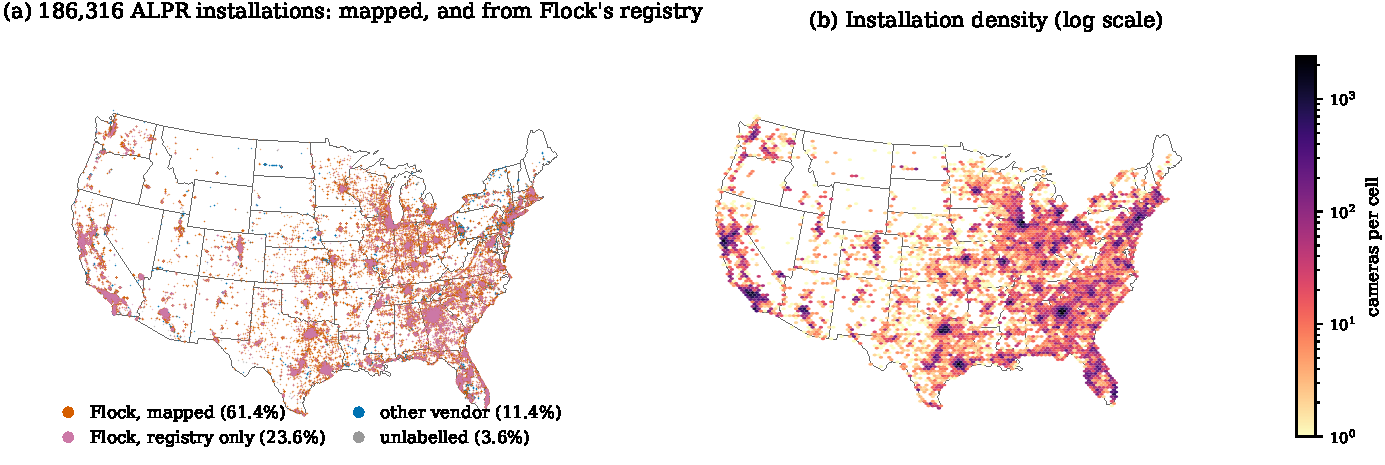
\includegraphics[width=\linewidth]{figures/fig_camera_map.pdf}
\caption{Mapped \alpr installations in the contiguous United States, 22 September 2026. (a) By
vendor: Flock Safety dominates by count almost everywhere. (b) Density on a log scale. The
visible structure is partly deployment and partly \emph{mapping}: see
\Cref{sec:results:coverage}. Camera data \textcopyright\ OpenStreetMap contributors.}
\label{fig:map}
\end{figure}

\subsection{Cone construction}
\label{sec:data:cones}

Each camera head becomes a circular sector: apex at the node, bisector along the tagged
bearing, span \ang{45} (or the tagged arc), radius \SI{60}{\metre}. The radius must reach
across the carriageway from a set-back pole; it was chosen on that reasoning and then swept
over $\{30,45,60,90\}\,\si{\metre}$ (\Cref{sec:lim:geom}). Measured exposure is only mildly
sensitive to it, but the avoidance result is not robust above the assumed value.

All wedges are unioned into a single MultiPolygon of \textbf{\num{135210} parts},
published as one feature with id \texttt{alpr}. Overlapping wedges merging is correct and
intended: the question is \emph{is this road segment observed}, not \emph{by how many
devices}.

\begin{table}[tbp]
\centering
\small
\caption{Vendor-split cone sets, 2026-09-22 snapshot; cameras are those with a bearing the
parser can read (\num{140043} of \num{142991}). The cones-per-camera column is itself a result:
non-Flock installations are multi-head more than six times as often (\SI{22.8}{\percent}
against \SI{3.6}{\percent}). A Flock unit typically watches one approach; other vendors' units
more often watch several lanes or directions.}
\label{tab:vendorsets}
\begin{tabular}{lrrrr}
\toprule
Set & Cameras & Cones & Cones/camera & Union parts \\
\midrule
Flock Safety       & \num{113611} & \num{120366} & 1.06 & \num{109427} \\
Other named vendor & \num{20435}  & \num{30128}  & \textbf{1.47} & \num{21587} \\
No vendor tag      & \num{5997}   & \num{6590}   & 1.10 & \num{5211} \\
\bottomrule
\end{tabular}
\end{table}

Assigning vendor requires care. Vendor appears under four keys
(\texttt{manufacturer}, \texttt{surveillance:\allowbreak manufacturer}, \texttt{brand},
\texttt{surveillance:\allowbreak brand}) and is spelled inconsistently. An exact match on
\texttt{manufacturer = "Flock Safety"} finds \num{109892} cameras; a case-insensitive
substring match on the first of the four keys present finds \num{114360}. The \num{4468}
difference is \num{3866} nodes that give the vendor only under \texttt{brand}, 599 that spell
the manufacturer differently (478 of them ``Flock Group Inc.''), and 3 that use
\texttt{surveillance:\allowbreak manufacturer}. Misfiling \SI{3.9}{\percent} of Flock cameras
as non-Flock is the one error a vendor comparison cannot absorb.

Untagged cameras are held out of \emph{both} vendor sets rather than assigned to the
complement of Flock: an untagged camera may well be an unlabelled Flock unit. They are reported as their own set so nothing is silently dropped,
with the caveat that their direction coverage is lower (\SI{88.0}{\percent} against
\SI{99.4}{\percent} for Flock and \SI{93.8}{\percent} for other named vendors---the last
down from \SI{98.5}{\percent} in July, as newly mapped Axis units often arrive without a
bearing).

\subsection{Camera maps of earlier dates}
\label{sec:data:history}

OpenStreetMap keeps every edit, so the camera map can be reconstructed as it stood on any
past date. The public Overpass server answers a query carrying a \texttt{[date:\ldots]}
qualifier from its history: nodes deleted since are restored, nodes added since are absent,
and every tag has its value from that day. Asked for Georgia at the July snapshot's
timestamp it returned \num{9742} nodes, the snapshot's own count to the node. History
queries for the whole continent time out on the public server, so a date is
fetched state by state and merged by node identifier; DeFlock's own Overpass mirror keeps
no history and cannot serve them. They are heavy, and after one complete date the public
server began refusing our connections.

The remaining dates were therefore reconstructed locally, from OpenStreetMap's full-history
dump \citep{osmplanet} (\SI{163}{\giga\byte}, 14 September 2026, checked against its published MD5), with
Overpass's semantics: every version of every node that was ever tagged as an \alpr,
including the later versions that deleted or retagged it, and for each date the latest
version at or before midnight UTC, kept if it was visible and still tagged. On the one date
both sources cover, 1 July 2025, they agree exactly---\num{22690} nodes, the same
identifiers, the same tags, the same coordinates.

We reconstruct five dates---1 January and 1 July of 2024 and of 2025, and 1 January
2026---and set them beside the study's July and September 2026 snapshots, seven maps in
all. Cones are built from each exactly as from the current map (\Cref{sec:data:cones}).
The share of mapped cameras carrying a bearing, and so receiving a cone, was about
\SI{90}{\percent} in 2024 and \SI{98}{\percent} in 2026: the earliest maps are slightly
less complete even on their own terms. Monthly counts between the dates come from
the ohsome history API \citep{raifer2019}, which aggregates but will not release individual records; it
agrees with our July snapshot to 21 nodes, exactly the readers tagged lowercase
\texttt{alpr} that the July fetch's case-sensitive match omitted.

One caveat governs everything built on these maps. OpenStreetMap records when a camera was
\emph{mapped}, not when it was installed: an installation date is present on 47 of
\num{142991} nodes. A camera first mapped in 2026 may have been on its pole since 2021. A
past map is therefore what a study run on that day would have seen, and the trend of
\Cref{sec:results:trend} describes how the measured picture changed as volunteers filled
in the map---most of it after DeFlock was founded in October
2024~\citep{deflock}---not how fast cameras were deployed.

\subsection{Road network}
\label{sec:data:roads}

Geofabrik North America extract \citep{geofabrik}, \SI{18}{\giga\byte}, retrieved 2026-07-24 and held
fixed for every camera map, so that the trend of \Cref{sec:results:trend} isolates the
camera data: every unavoided route is the same route on every date. Imported with
\texttt{ignored\_highways = footway,\allowbreak construction,\allowbreak cycleway,\allowbreak path,\allowbreak steps}. \texttt{track} is
deliberately retained: unpaved tracks are plausible avoidance routes, and excluding them
would bias the cost estimate downward by removing options a determined driver has.

Traffic, used to weight the siting comparison of \Cref{sec:results:siting} by
vehicle-kilometres, comes from FHWA's Highway Performance Monitoring System for 2024
\citep{hpms2024}: the annual average daily traffic of every section of the federal-aid
network, which each state must report for all of its Interstates, freeways, arterials and major
collectors. We keep those classes and drop the non-inventory direction of divided roads---the
second carriageway, which HPMS maps but does not count separately, its traffic being included in
the other's---so that each road is counted once, at its two-way volume. The result, \num{1.68}~million kilometres, carries \num{2849}~billion
vehicle-miles a year in the fifty states and DC, \SI{87}{\percent} of the \num{3279}~billion
FHWA estimates for all roads and streets in 2024 \citep{fhwa2025tvt}.

\subsection{Commute sample}
\label{sec:data:commutes}

Source: LEHD \textbf{LODES8} \citep{lodes8}, file \texttt{od\_main\_JT00}: all jobs with both
ends in-state, built from unemployment-insurance wage records linked to employer
establishments. These are
administrative counts of real jobs, not survey estimates. The year is 2022, the last year of
the ACS estimates the demographics come from, for 49 of the 51 jurisdictions; LODES has not published 2022 for Michigan, which uses 2021, or for Alaska,
whose latest year is 2016. LODES8 codes every year against 2020 census geography, so an
older year still names current tracts.

Sampling design carries more weight here than sample size. Uniform random points would
over-represent empty rural space where nobody commutes and no cameras exist, understating
exposure badly. Instead each origin--destination pair is drawn \textbf{with probability
proportional to the number of workers actually making that trip}, so the distribution
approximates what an average \emph{commuter} experiences rather than what an average
\emph{square kilometre} contains.

Block-level LODES geocodes are aggregated to \textbf{tract} (first 11 digits)---the finest
resolution at which ACS demographics are reliable, and finer than the routing's effective
precision. Same-tract commutes are dropped: origin and destination centroids coincide, so
there is no route to measure. Georgia alone yields \num{1199250} distinct tract pairs
covering \num{4190313} workers; across the 50 states and the District of Columbia the frame
holds \num{132822679} commuters over \num{34420305} tract pairs.

Connecticut needed one repair. In 2022 it replaced its eight counties with nine planning
regions, and every tract identifier changed with them. LODES still names tracts by the old
counties while the 2024 Gazetteer and ACS 2022 use the new ones, so without a crosswalk no
Connecticut tract matches and the state silently drops out of the sample. The tracts were
reassigned, not redrawn: each six-digit tract code maps to exactly one new identifier, and
all 879 in the flows do.

\num{1200} pairs are drawn per jurisdiction, \num{61200} in all, with replacement from a
single seeded stream (seed \texttt{20260725}), giving \textbf{\num{58421} distinct commutes}.
The fifteen states of the study's earlier rounds are drawn first, so their \num{17904}
commutes are reproduced exactly and their routes carry over. The sampled pairs represent
\num{2842747} workers; the median pair carries 16 and the largest \num{2832}.

A pair drawn more than once is routed once, since its route is the same, but it stands for
every draw: \textbf{each commute carries its draw count as a weight}. In the fifteen large
states this is immaterial---\SI{0.53}{\percent} of draws are repeats---but in small ones it
is not. Wyoming's \num{1200} draws hold 832 distinct pairs (\SI{30.7}{\percent} repeats),
Alaska's repeat a quarter of the time and the Dakotas' nearly a fifth, and one Vermont pair was
drawn nine times. Collapsing repeats at equal weight, as this study's earlier rounds did,
under-represents precisely the heaviest flows; keeping the counts restores
probability-proportional-to-workers sampling inside every state.

\subsection{Demographics and geography}

Tract centroids are 2024 Census Gazetteer internal points \citep{gazetteer2024}
(\texttt{INTPTLAT}/\texttt{INTPTLONG}), which are guaranteed to fall inside the tract
polygon. Income is ACS 5-year 2018--2022 \citep{acs2022} table \textbf{B19013}; race and ethnicity are table
\textbf{B03002}, chosen over B02001 because it is Hispanic-aware, so ``non-Hispanic
Black'' is directly available rather than reconstructed. Demographics attach to the
\emph{origin} (home) tract: the claim under test concerns who lives where surveillance is
dense.

\section{Method}
\label{sec:method}

\subsection{Two routes per commute}

Each sampled pair is routed twice against the same graph: a \textbf{baseline} with no
custom model, and an \textbf{avoided} route applying
\texttt{priority: [\{if: "in\_alpr", multiply\_by: 0.01\}]}. Both disable CH, which
per-request custom models require.

Both use GraphHopper's stock car model, which weighs distance as well as time
(\texttt{distance\_\allowbreak influence} 90: a route \SI{1}{\kilo\metre} shorter is preferred if it
costs under \SI{90}{\second} more). The baseline is therefore the router's preferred route
rather than strictly the fastest, and for \SI{4.5}{\percent} of commuters the avoiding
route---in every such case the longer one---is the quicker, by a median of
\SI{0.9}{\minute}. Extra time is reported as measured, negative values included; clipping
them at zero leaves every median unchanged and raises the mean extra time from
\SI{5.62}{\minute} to \SI{5.70}{\minute}.

\num{0.01} is the application's \emph{strongest} avoidance setting, not a typical one: a
watched road costs a hundred times its usual weight, close to but short of prohibition.
Results therefore describe the \textbf{strong end of both the benefit and the cost} of
avoidance as offered. This is deliberate: it establishes whether meaningful avoidance is
possible at all, and what it costs near the limit.

\subsection{Exposure is directional, not proximate}

A camera counts as having seen the driver \emph{only if the route line intersects its
cone}. Passing \SI{20}{\metre} from a camera aimed the other way is not exposure.
Implementation is an STRtree over the \num{135210} cone parts for candidate lookup, then
an exact intersection test.

Two simplifications remain, and they pull in opposite directions: route geometry is a
polyline while a vehicle has width, which understates exposure, and a cone occluded by
intervening buildings is still counted as full sight-line, which overstates it.

\subsection{Vendor attribution costs no additional routing}

Routing does not change between vendor questions---the avoidance model targets the
all-vendor union either way---so \Cref{sec:results:vendor} is entirely a matter of
re-scoring existing routes against different cone sets. This is possible only because the
experiment persists route polylines to a sidecar; keeping only counts would have made both
the vendor split and the radius sweep of \Cref{sec:lim:geom} fresh multi-hour re-runs.

As a consistency check, the three vendor sets should sum to slightly \emph{more} than the
all-vendor union, because cones from different vendors that overlap merge into one part in
the union and are counted once while the split sets count them separately. Measured excess
is \SI{1.0}{\percent}: right sign, plausible magnitude.

\subsection{Earlier camera maps need no new baselines}
\label{sec:method:history}

The unavoided route does not depend on the cameras. Routed two months apart against graphs
carrying different camera maps, all \num{17580} commutes of the study's earlier rounds took
identical baseline routes, to the metre and the second. Exposure on an earlier date is
therefore a re-scoring of each saved route against that date's cones, with no routing.

Avoidance does need routing against that date's cameras, and two properties keep it
tractable. First, one graph serves every date: each date's cone set is imported as its own
custom area (\texttt{alpr\_2025\_07\_01}, \ldots), and each request names the one it avoids
---a single import of about two hours rather than one per date, checked on a test graph to
route each area independently. Second, only commutes that pass a camera on that date are
routed. A route that crosses no cone is already the avoiding route, since the custom model
only makes cone edges dearer and nothing can undercut it; this was checked rather than
assumed, and all \num{3741} such commutes of the fifteen-state run received an identical
avoiding route. The same shortcut serves the main run.

Re-scoring uses route geometry stored at five decimal places, about a metre. Against live
scoring on the current map it moves \SI{1.7}{\percent} of commutes by one camera, in the two
directions about equally, changes whether 5 of \num{17580} (\SI{0.03}{\percent}) pass any
camera at all, and leaves national totals within \SI{0.1}{\percent}. On the full sample the
re-scored national figures match the live ones to the precision reported
(\SI{75.3}{\percent} passing a camera, a mean of \num{5.14}). Within the trend every date,
the current one included, is scored the same way. The July 2026 snapshot enters the trend
re-scored only: routing its avoidance in all fifty-one states would have added most of a day
of computation to a step that the fifteen-state paired comparison already covers
(\Cref{sec:results:trend}).

\subsection{Statistical reporting}
\label{sec:method:stats}

\begin{itemize}
  \item \textbf{Medians lead, means accompany.} Both distributions are heavily
    right-skewed; a minority of long commutes through dense corridors pull the mean well
    above the typical experience.
  \item \textbf{National figures are weighted by commuters.} Every jurisdiction was sampled
    at the same size, so an unweighted pool would count Wyoming's \num{198447} in-state
    commuters as heavily as California's \num{16821903}. Each routed commute carries its
    state's commuter total from the LODES frame, shared among that state's routed commutes in
    proportion to draw count, and quartile cut-points and medians are weighted quantiles.
    State figures are within-state estimates and need only the draw counts. The weights
    matter even on the fifteen states of the earlier rounds: weighting alone moves the share
    of commuters passing a reader there from \SI{78.7}{\percent} to \SI{81.1}{\percent},
    because the populous states are the more surveilled ones.
  \item \textbf{Confidence intervals from a bootstrap stratified by state}
    \citep{efron1993} (percentile, \num{2000} replicates, seed \texttt{20260725}). Each
    replicate resamples every state at its own size and re-derives its weights, as the sample
    was drawn; a plain bootstrap over pooled rows would let one replicate hold \num{1400}
    Texans and 900 Californians, variation the design does not have. Camera counts are
    discrete and zero-inflated, nowhere near normal, so no interval is assumed symmetric.
  \item \textbf{Commutes from one county are not independent.} They share corridors, and so
    cameras, and a bootstrap over commutes treats them as independent. Resampling whole origin
    counties within states instead \citep{field2007} widens the intervals on the headline
    figures two- to threefold---\SI{75.3}{\percent} of commuters passing a reader becomes
    [74.0--76.4], the median extra time of \SI{1.62}{\minute} [1.48--1.84]---and on the
    national contrasts about twofold. On the current map it leaves every contrast of
    \Cref{sec:results:demo,sec:results:coverage,sec:results:vendor} on the same side of parity
    except two already on the line; on the sparse early maps it matters more
    (\Cref{sec:results:trend}). Where the two bootstraps disagree about parity, both are
    shown. The siting analysis resamples counties throughout.
  \item \textbf{A contrast is distinguishable when the interval on its ratio excludes
    parity} under both bootstraps. Earlier rounds of this study asked instead that the
    intervals on the two quartile means not overlap, a criterion far stricter than a
    \SI{5}{\percent} test \citep{schenker2001}; on the current map the two give the same
    verdict on every contrast of
    \Cref{sec:results:demo,sec:results:coverage,sec:results:vendor}.
  \item \textbf{Many contrasts are reported.} The two siting hypotheses and the exposure
    contrasts were posed before their analyses were run; the vendor, operator, edge and
    boundary contrasts are descriptive, and one interval that narrowly excludes parity among
    them should be read as such. The headline siting contrasts are far from that line: of the
    24 by race, ethnicity and income for arterial, residential and police-operated cameras and
    per vehicle-kilometre, in both schemes, 22 have no county-bootstrap replicate beyond parity
    ($p<0.001$), which survives a Bonferroni correction for all 24; the other two are Hispanic
    contrasts within county and density band, for police-operated cameras ($p\approx0.015$)
    and per vehicle-kilometre ($p\approx0.003$).
  \item \textbf{Quartile contrasts, not regressions.} A ratio of the highest quartile to the
    lowest assumes no functional form, reads directly, and is the same comparison for exposure
    and for siting. Like a regression coefficient it describes an association, not an effect.
  \item \textbf{Total exposure and per-kilometre density are reported as peers.} A raw
    count gap that vanishes once normalised per km is about distance, not siting. But the
    converse is a finding, not a nuisance: a group whose commutes are \emph{shorter but
    more densely watched} shows a rate gap and no count gap, and treating the rate purely
    as a control would discard it. Cameras per km is a ratio of sums bootstrapped over
    commutes; a mean of per-commute rates would let very short commutes dominate.
  \item \textbf{Ecological inference is not attempted.} Tract composition is a property of
    tracts, not of the individuals routed.
\end{itemize}

\subsection{Execution}
\label{sec:method:exec}

Twelve concurrent workers against the local routing server. Worker count was measured, not
assumed: twelve completed 300 commutes in \SI{324}{\second}, while thirty-two took longer
than \SI{576}{\second} on the identical set---past about twelve, contention outweighs added
concurrency. Routing dominates cost overwhelmingly; the geometric exposure test is
\SI{0.2}{\percent} of per-commute work.

Failed routes are dropped rather than retried, and \textbf{\num{56131} of \num{58421}
commutes routed (\SI{3.9}{\percent} dropped)}. The failures are not spread evenly, and not
mostly what they seem. Nine in ten are points the router cannot snap to any road: a tract's
internal point can lie deep inside a national park, a reservation or a wilderness tract,
beyond the router's road search. The rest are genuinely unconnected---commutes between
Hawaiian islands, or to Alaskan towns off the road network. Five states lose more than a
tenth of their sample (Alaska \SI{33}{\percent}, Hawaii \SI{24}{\percent}, Montana and
Wyoming \SI{21}{\percent}, New Mexico \SI{14}{\percent}); the median state loses
\SI{2.0}{\percent}. Those five hold \SI{1.6}{\percent} of the nation's commuters, so the
national figures barely register the loss, but their own estimates describe the routable
part of each state---probably its less remote part, and so probably overstate its
exposure. A wider road search would recover most of them, but it also moved 5 of 100
already-routed commutes to a different road (the default search sometimes stops at a road
that is not the nearest), and the trend of \Cref{sec:results:trend} pairs every saved route
with new ones. Consistency was kept over coverage.

Commutes are processed in seeded random order. The sample is grouped by state and the
executor preserves input order, so in file order results arrive one state at a time: an
interruption would leave some states complete and others absent, and no partial output
could support a national estimate. Shuffling makes any prefix a near-uniform sample of the
whole. This proved material rather than hypothetical---in the study's first round an
interim read of a single state gave a median avoidance overhead of \SI{22.7}{\percent}
against that round's national \SI{5.96}{\percent}.

\section{Results}
\label{sec:results}

\subsection{Exposure on the unavoided commute}
\label{sec:results:exposure}

\begin{table}[tbp]
\centering
\small
\caption{Exposure and the cost of avoidance for American commuters: \num{56131} routed
commutes in the 50 states and the District of Columbia, weighted to the \num{132.8}
million in-state commuters they represent. Medians are weighted; intervals come from a
bootstrap stratified by state. Median commute \SI{23.6}{\kilo\metre} / \SI{23.4}{\minute}.}
\label{tab:headline}
\begin{tabular}{lrr}
\toprule
& Median [\SI{95}{\percent} CI] & Mean \\
\midrule
\multicolumn{3}{l}{\itshape Unavoided route} \\
Cameras passed              & 3 [3--3]            & 5.14 \\
Commuters passing $\geq$1   & \multicolumn{2}{r}{\SI{75.3}{\percent} [74.8--75.8]} \\
Commuters passing $\geq$5   & \multicolumn{2}{r}{\SI{36.5}{\percent}} \\
Commuters passing $\geq$10  & \multicolumn{2}{r}{\SI{16.3}{\percent}} \\
\nth{90} / \nth{99} percentile & \multicolumn{2}{r}{13 / 34 cameras} \\
Exposure rate               & \multicolumn{2}{r}{\num{0.096} cameras/\si{\kilo\metre}} \\
\midrule
\multicolumn{3}{l}{\itshape ALPR-avoiding route} \\
Cameras passed              & 0 [0--0]            & 0.26 \\
\textbf{Reduced to zero}    & \multicolumn{2}{r}{\textbf{\SI{84.2}{\percent}} [83.7--84.7]} \\
Extra time (\si{\minute})   & \textbf{1.62} [1.57--1.68] & 5.62 \\
Extra distance (\si{\kilo\metre}) & 0.57 [0.55--0.60] & 2.53 \\
Avoidance overhead          & \SI{6.71}{\percent} [6.50--6.93] & \SI{13.27}{\percent} \\
Minutes per camera evaded   & 0.76 [0.75--0.78]   & 1.30 \\
\bottomrule
\end{tabular}
\end{table}

\begin{figure}[tbp]
\centering
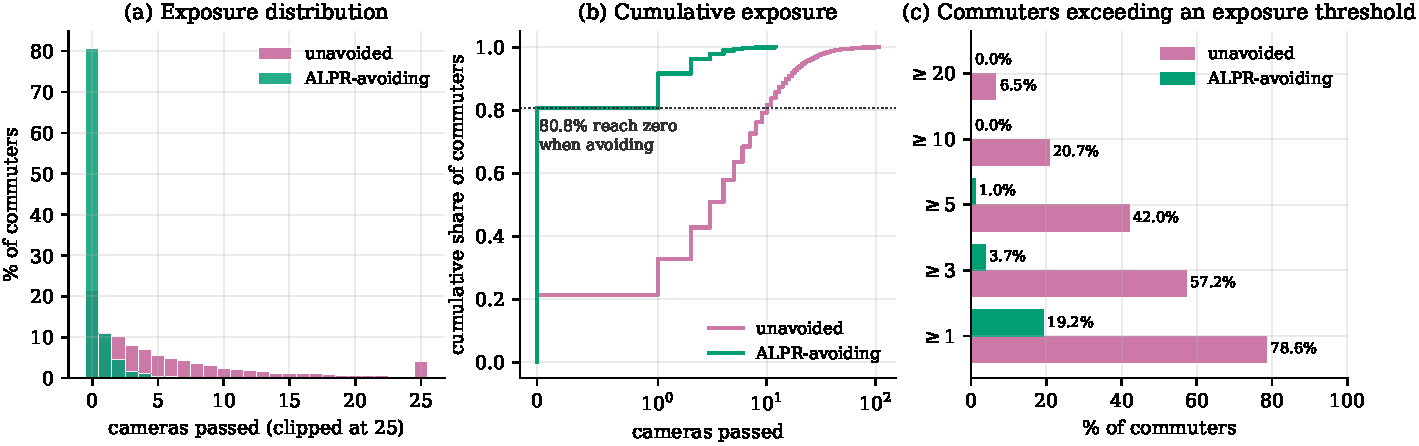
\includegraphics[width=\linewidth]{figures/fig_exposure.pdf}
\caption{Exposure before and after \alpr-avoiding routing, as shares of commuters. (a)
Distributions; (b) cumulative, log-scaled abscissa; (c) share of commuters exceeding a
threshold. The zero-exposure mass moves from \SI{24.7}{\percent} to \SI{84.2}{\percent}.}
\label{fig:exposure}
\end{figure}

\textbf{\SI{75.3}{\percent} of American commuters pass at least one \alpr} on the way to
work. The median commuter passes three, the \nth{90} percentile thirteen and the \nth{99}
thirty-four. Aggregate exposure is \num{0.096} cameras per
kilometre driven. Across the fifteen states of the study's earlier rounds the same weighted
share is \SI{81.1}{\percent}: the thirty-five states and the District added here are, on
the map, far less surveilled---a difference \Cref{sec:results:geo,sec:results:coverage}
will not let us attribute to the roads rather than to the map.

\subsection{The cost of refusal}
\label{sec:results:cost}

\begin{figure}[tbp]
\centering
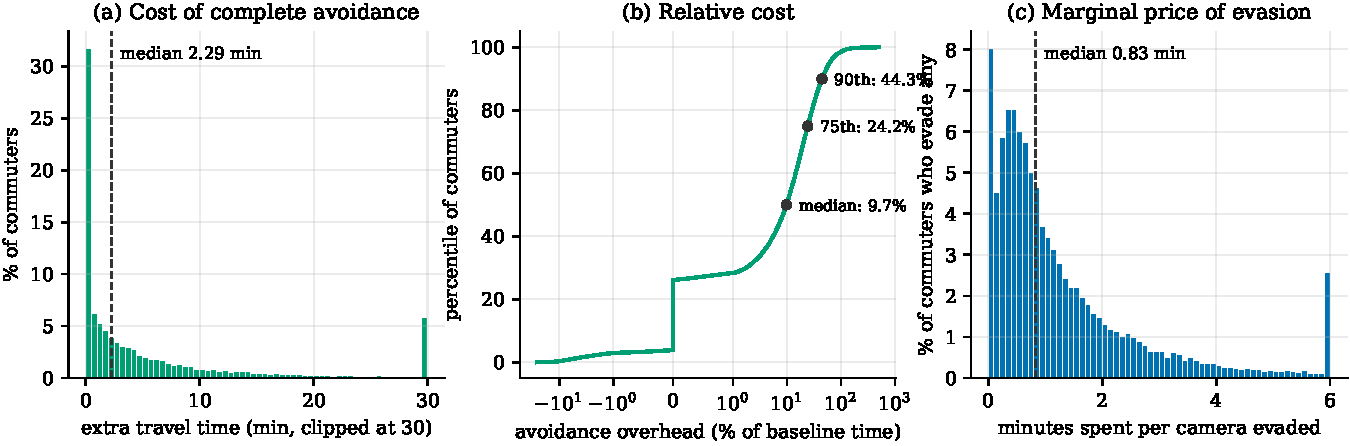
\includegraphics[width=\linewidth]{figures/fig_cost.pdf}
\caption{The price of complete avoidance, as shares of commuters. (a) Absolute extra time;
(b) overhead as a percentage of baseline, by percentile; (c) marginal minutes per camera
evaded. All three are heavily right-skewed---a small tail of commutes pays a great deal,
while the typical commute pays almost nothing.}
\label{fig:cost}
\end{figure}

\textbf{\SI{84.2}{\percent} of American commuters could be routed to zero \alpr
exposure}: the quarter whose usual route passes no mapped reader, and four in five of the rest
(\SI{79.0}{\percent} [78.4--79.7], \Cref{tab:trend}). Over all commuters the avoiding route
adds a median of \SI{1.62}{\minute} and \SI{0.57}{\kilo\metre}, an overhead of
\SI{6.71}{\percent}; for commuters whose usual route passes a camera it adds a median of
\SI{3.14}{\minute} [3.05--3.22]. The median marginal price is \SI{0.76}{\minute} per camera
evaded.

For most commuters, then, refusing licence-plate surveillance on the way to work costs a few
minutes at most. This is conditional on the assumed camera field of view: it is stable if the
true radius is smaller than the \SI{60}{\metre} assumed here and degrades if it is
substantially larger, which \Cref{sec:lim:geom} quantifies. It is the paper's central
quantitative claim.

The distribution matters as much as the median. The mean overhead is \SI{13.27}{\percent}
against a median of \SI{6.71}{\percent}, and the interquartile range runs from
\SI{0}{\percent} to \SI{18.9}{\percent}: a quarter of commuters need no detour whatsoever,
while a tail pays substantially. \Cref{fig:route} shows one such case.

\begin{figure}[tbp]
\centering
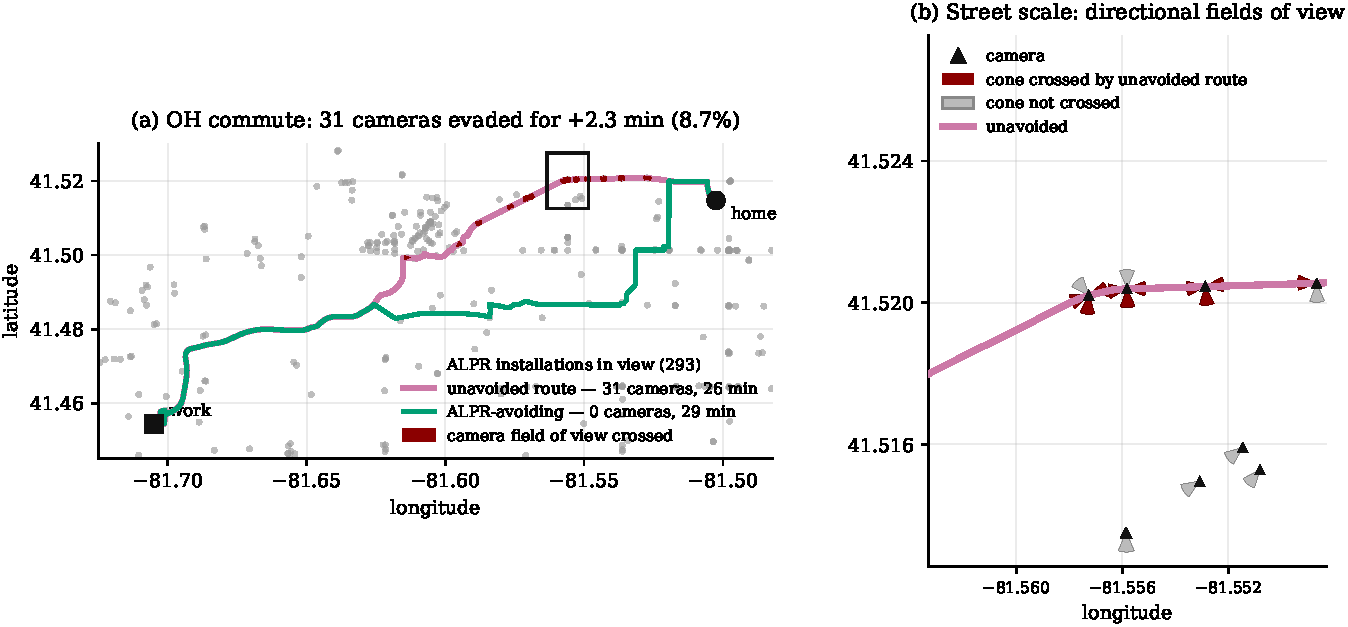
\includegraphics[width=\linewidth]{figures/fig_route_example.pdf}
\caption{An illustrative high-exposure commute in the Cleveland area---chosen for
legibility, not typicality. (a) The unavoided route crosses 31 camera fields of view; the
avoiding route crosses none, for \SI{+2.3}{\minute} (\SI{8.7}{\percent}). (b) At street scale the
directional model is visible: cones the unavoided route crosses are dark, cones aimed
elsewhere are grey and cost nothing. Map data \textcopyright\ OpenStreetMap contributors.}
\label{fig:route}
\end{figure}

\subsection{Fifty states and the District of Columbia}
\label{sec:results:geo}

\begin{figure}[tbp]
\centering
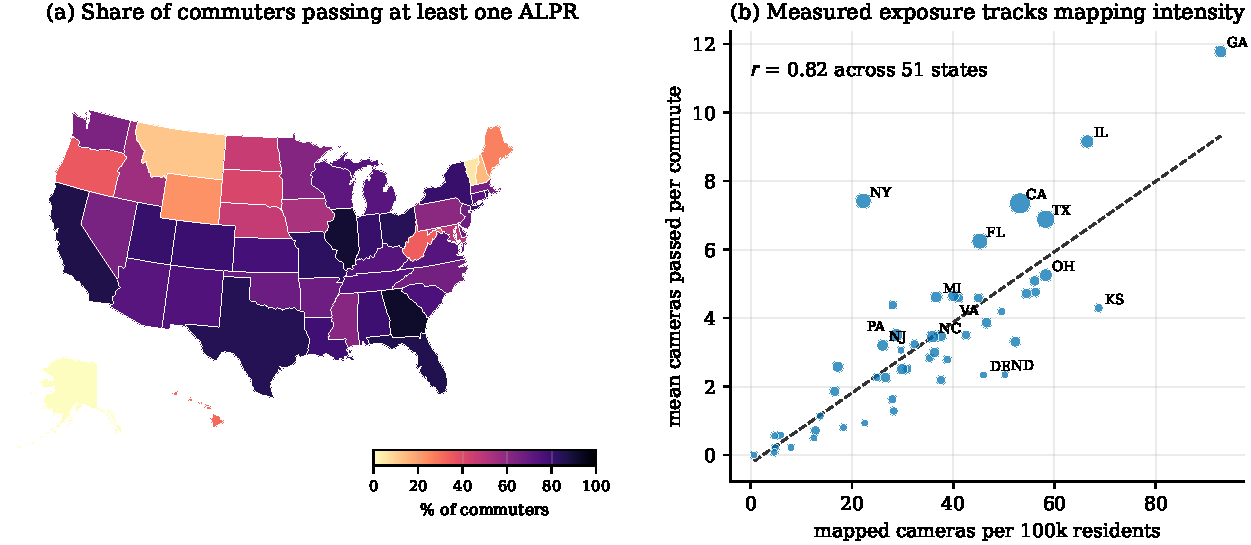
\includegraphics[width=\linewidth]{figures/fig_states.pdf}
\caption{(a) Share of each state's commuters whose unavoided route passes at least one
mapped \alpr. (b) Mean cameras passed against mapped cameras per \num{100000} residents,
points sized by commuters. Mapping intensity alone tracks most of the variation between
states ($r=0.82$)---the central interpretive problem of \Cref{sec:results:coverage}.}
\label{fig:states}
\end{figure}

State-level variation is extreme (\Cref{fig:states}; every state is tabulated in
\Cref{tab:bystate}). In Georgia \SI{91.9}{\percent} of commuters pass a mapped reader, a
mean of \num{11.8} on the way to work, and avoiding them costs a median \SI{25.7}{\percent} overhead;
in Illinois \SI{90.6}{\percent} do, in California \SI{86.7}{\percent}. At the other end
\SI{14.8}{\percent} of New Hampshire's commuters pass one, \SI{11.8}{\percent} of
Montana's, \SI{5.4}{\percent} of Vermont's, and none of Alaska's sampled commuters. In
fifteen jurisdictions the median extra time is zero: most of their commuters have nothing
on the map to avoid.

These are differences in the map at least as much as on the roads. Mapped density runs
from \num{0.7} cameras per \num{100000} residents in Alaska, and under five in Vermont,
Maine and New Hampshire, to \num{92.8} in Georgia---a \num{7.1}-fold spread between the
\nth{10} and \nth{90} percentile states---and state exposure tracks it at $r=0.82$. The
departures from the line are what a statewide rate would produce: New York's commuters pass
more cameras than its statewide density predicts, because commuting concentrates where
cameras do while the density is averaged over the whole state; Kansas's pass fewer.

Per camera, evasion tends to be cheaper where cameras are denser. Across the 48 states with
at least 100 evading commuters, the median price per camera falls as cameras per kilometre
rise ($r=-0.29$ against the logarithm of cameras per kilometre, \SI{95}{\percent} CI $-0.53$ to
$-0.01$), from \SI{2.49}{\minute} in New Hampshire to
\SI{0.17}{\minute} in the District of Columbia. Dense grids offer a parallel street one
block over; rural and intercity routes often have one road. Across states the relationship
is weak---Georgia, the most densely watched
large state, still pays \SI{1.11}{\minute} a camera---so we state it as a tendency, not a
law: the burden of refusal falls, if anything, hardest on drivers with the fewest cameras
to refuse.

\subsection{Demographic contrasts}
\label{sec:results:demo}

\begin{figure}[tbp]
\centering
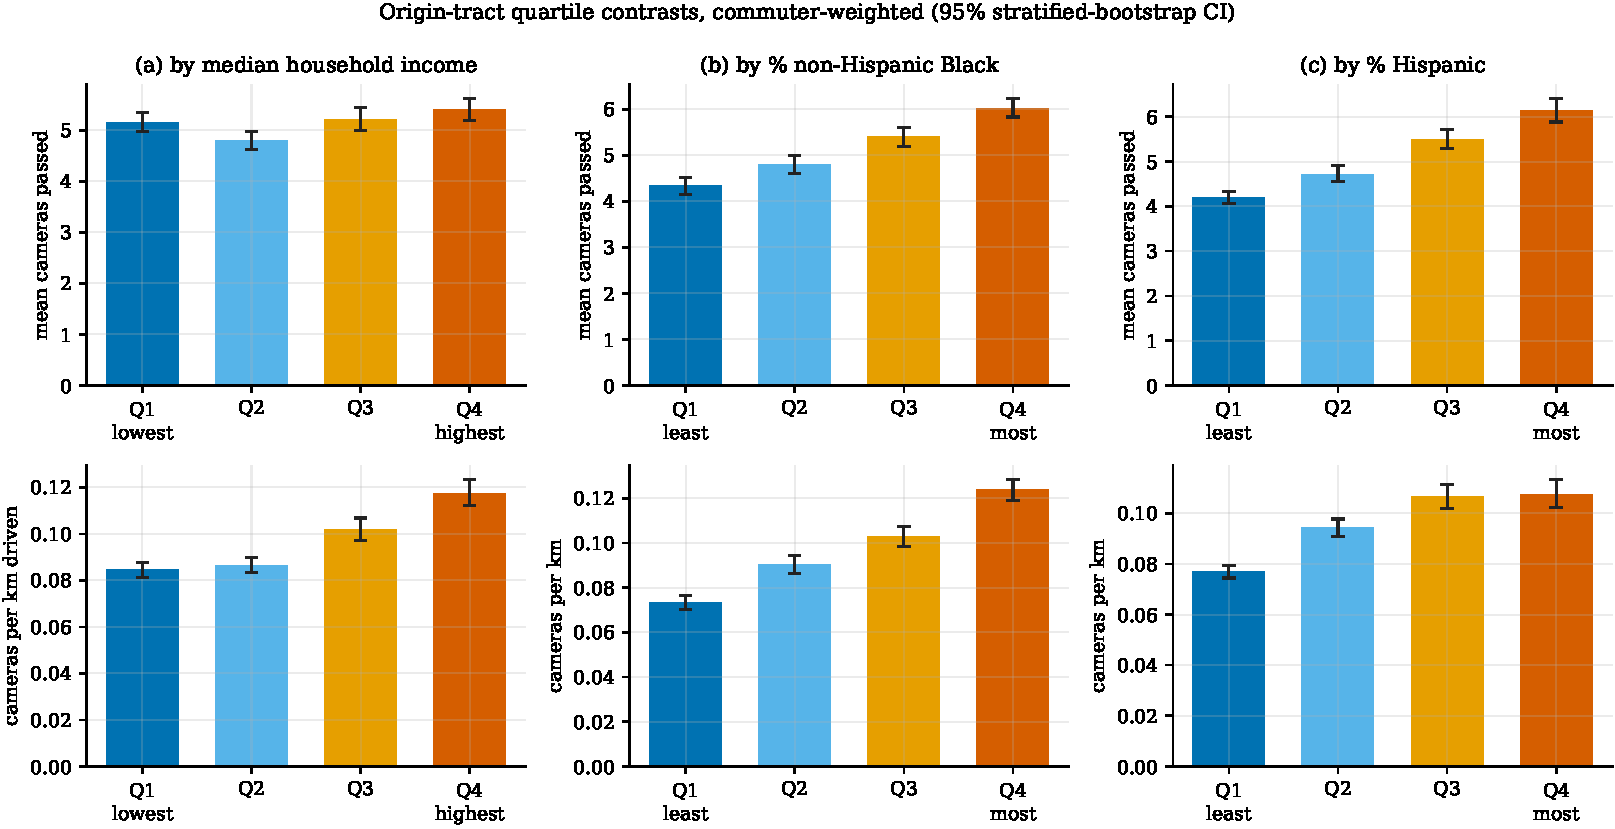
\includegraphics[width=\linewidth]{figures/fig_demographics.pdf}
\caption{Origin-tract quartile contrasts, commuter-weighted, with \SI{95}{\percent}
stratified-bootstrap intervals. Top row: mean cameras passed. Bottom row: cameras per
kilometre driven. Income shows a per-km gradient with no count gradient---higher-income
origins have denser commutes, shorter on average.}
\label{fig:demo}
\end{figure}

\begin{table}[tbp]
\centering
\small
\caption{National quartile contrasts, commuter-weighted: the highest quartile of origin tracts
over the lowest (for income, the richest over the poorest), in mean cameras passed and in
cameras per kilometre driven. \SI{95}{\percent} intervals from the stratified bootstrap and,
beneath them, from one that resamples whole origin counties (\Cref{sec:method:stats}); bold
marks a ratio whose interval excludes parity under both. Cameras per kilometre, lowest against
highest quartile: income \num{0.0846} against \num{0.1174}, Black \num{0.0733} against
\num{0.1238}, Hispanic \num{0.0769} against \num{0.1074}.}
\label{tab:demo}
\begin{tabular}{lcc}
\toprule
Highest over lowest quartile & Mean cameras passed & Cameras per km driven \\
\midrule
Income (richest over poorest)  & 1.05 [0.99--1.11]            & \textbf{1.39} [1.31--1.48] \\
\quad resampling counties      & [0.95--1.19]                 & [1.27--1.63] \\
\% non-Hispanic Black          & \textbf{1.39} [1.32--1.47]   & \textbf{1.69} [1.59--1.78] \\
\quad resampling counties      & [1.27--1.53]                 & [1.55--1.91] \\
\% Hispanic                    & \textbf{1.46} [1.39--1.54]   & \textbf{1.40} [1.32--1.48] \\
\quad resampling counties      & [1.34--1.63]                 & [1.26--1.58] \\
\bottomrule
\end{tabular}
\end{table}

Both ethnic and racial contrasts are statistically distinguishable nationally, and the
Hispanic one is now the larger: commuters from the most Hispanic quartile of origin tracts
pass \num{1.46} times as many cameras as those from the least. Income is not
distinguishable in counts---but higher-income origin tracts show materially \emph{denser}
per-kilometre exposure (\num{0.1174} against \num{0.0846}, \num{1.39}$\times$) offset by
commutes that are shorter on average. Only reporting count and rate as peers surfaces that; a design treating the rate as a mere
control would have discarded it.

\subsection{Coverage-bias sensitivity, and why it governs the reading}
\label{sec:results:coverage}

\begin{figure}[tbp]
\centering
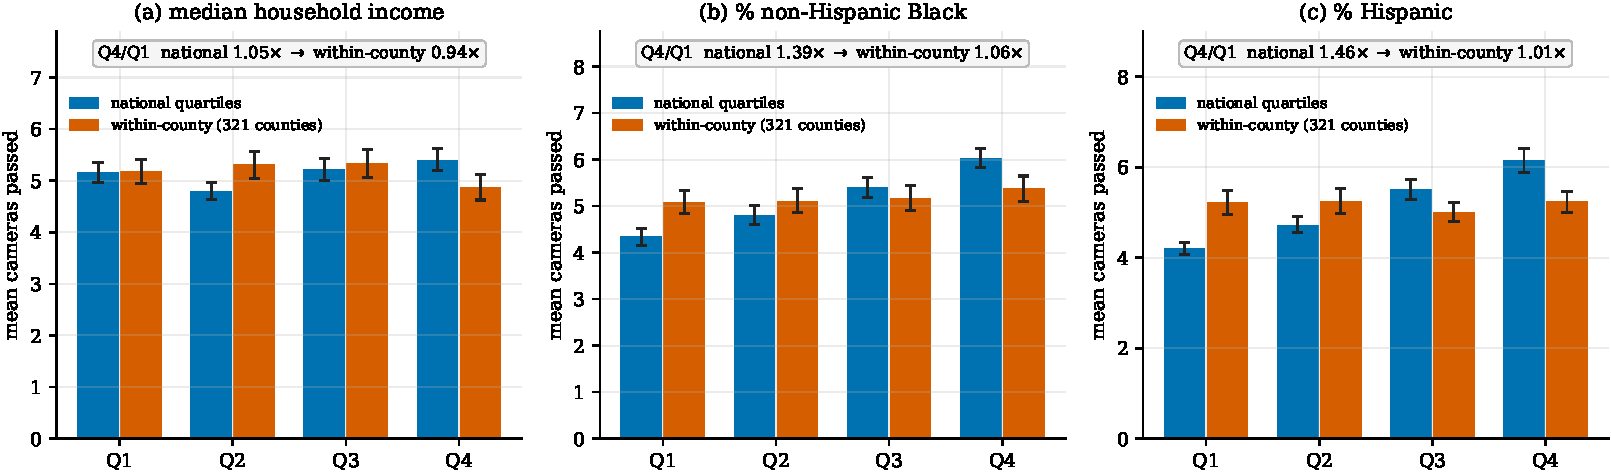
\includegraphics[width=\linewidth]{figures/fig_within_county.pdf}
\caption{The central negative result for exposure. Ranking origin tracts within their own
county rather than nationally collapses every demographic gradient in commute exposure to
indistinguishability. \num{321}
counties with $n\geq40$ contribute \SI{68}{\percent} of the sample and \SI{63}{\percent} of
its commuters.}
\label{fig:within}
\end{figure}

\Cref{fig:within} is the most consequential figure for reading the exposure results.
Recomputing quartiles
\emph{within each county} and pooling by commuters---so tracts are ranked only against
neighbours subject to the same local mapping effort and broadly the same urban form---
collapses every demographic gradient in exposure. The racial gradient falls from \num{1.39}$\times$
[1.32--1.47] to \num{1.06}$\times$ [0.99--1.13]; the Hispanic gradient, the largest
nationally, from \num{1.46}$\times$ to \num{1.01}$\times$ [0.94--1.08]; income stays
indistinguishable, its highest quartile against its lowest at \num{0.94}$\times$
[0.88--1.01]. Within-county per-kilometre rates are
close: \num{0.1163} against \num{0.1268} by racial composition.

On the current map the demographic gradients in commute exposure are therefore
\textbf{entirely a between-county phenomenon}---a statement that, as \Cref{sec:results:trend}
shows, could not have been made of the sparser maps before it, and one about what commuters
pass rather than where cameras stand (\Cref{sec:results:siting}).

The price of refusal follows the same pattern. Nationally, commuters from the most-Black
quartile of tracts would pay a median of \SI{1.94}{\minute} to avoid every camera, against
\SI{1.28}{\minute} from the least-Black (a difference of \num{0.66} [0.50--0.84], or [0.37--1.05]
resampling counties), and from the most-Hispanic \SI{1.89}{\minute} against \SI{1.33}{\minute}.
That is because they pass more cameras, not because each costs more: the median price per
camera evaded is lower for them (\SI{0.72}{\minute} against \SI{0.84}{\minute}, and
\SI{0.66}{\minute} against \SI{0.93}{\minute}), their cameras standing in the dense grids where a
detour is short (\Cref{sec:results:geo}). Within counties the difference in total cost vanishes:
\SI{1.44}{\minute} against \SI{1.61}{\minute} by Black share, \SI{1.58}{\minute} against
\SI{1.57}{\minute} by Hispanic share, and \SI{1.53}{\minute} for the richest quartile against
\SI{1.40}{\minute} for the poorest, with no difference distinguishable when counties are
resampled. Within a county, the price of refusal is evenly held.

Between states, exposure tracks mapped density (\Cref{sec:results:geo}), and from any single
map we cannot distinguish ``Pennsylvania has few cameras'' from ``Pennsylvania has few
mappers''; the map's history in \Cref{sec:results:trend} shows what can be said.

Three explanations remain consistent with these data, and this design cannot fully
separate them:
\begin{enumerate}
  \item \textbf{Differential mapping effort.} Volunteer contributors are unevenly
    distributed, and where they are absent cameras are absent from the map but present on
    the pole. The external check of \Cref{sec:results:siting} bounds this where police
    departments publish camera counts---there, how completely a city is mapped is unrelated
    to its Black share---but not between regions, or where no count is published.
  \item \textbf{Urban form.} High-\%Black and high-\%Hispanic tracts are disproportionately
    urban and urban roads carry more cameras per kilometre, so the national contrast is
    substantially an urban/rural contrast.
  \item \textbf{Genuine between-jurisdiction procurement differences.} Municipalities
    really do differ in what they buy.
\end{enumerate}

We therefore decline to report a national demographic finding in commute exposure as a
finding about surveillance siting. What we report here is narrower and defensible: a gradient
in exposure exists in the observable data, it is between-county, and it does not survive
local ranking. Siting is a different question, answered directly in \Cref{sec:results:siting}
---where, within counties, a gradient does appear.

\subsection{By camera vendor}
\label{sec:results:vendor}

\begin{figure}[tbp]
\centering
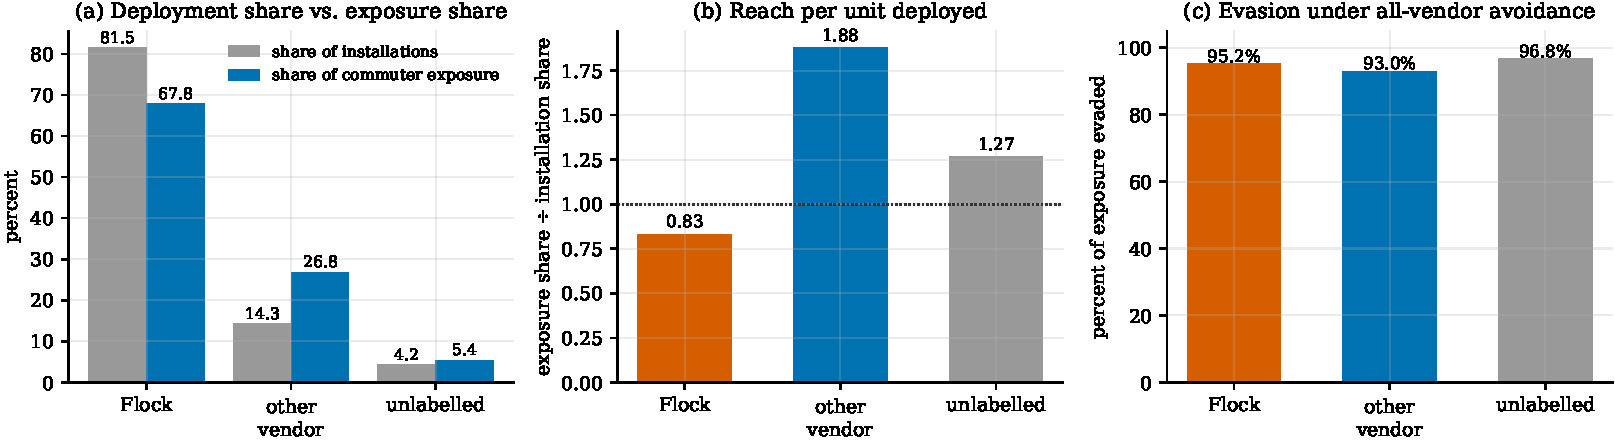
\includegraphics[width=\linewidth]{figures/fig_vendor.pdf}
\caption{Vendor-resolved exposure, commuter-weighted. (a) Flock's share of exposure falls
well below its share of installations. (b) Reach per unit deployed: share of exposure
divided by share of installations. (c) Both are avoided at comparable rates under the
all-vendor model. Installations are the cameras that contribute cones.}
\label{fig:vendor}
\end{figure}

\begin{table}[tbp]
\centering
\small
\caption{Vendor-resolved exposure, commuter-weighted over the 51-state sample. Installation
shares are of the \num{139391} cameras in the 50 states and the District of Columbia that
contribute cones. Reach is share of exposure divided by share of installations: Flock holds
four-fifths of installations and supplies two-thirds of exposure, and per unit deployed a
non-Flock camera generates \num{2.26}$\times$ as many camera encounters.}
\label{tab:vendorexp}
\begin{tabular}{lrrrrr}
\toprule
Set & Installations & Share of exposure & Reach & Commuters $\geq$1 & Evaded \\
\midrule
Flock Safety  & \SI{81.5}{\percent} & \SI{67.8}{\percent} & \num{0.83} & \SI{65.5}{\percent} & \SI{95.2}{\percent} \\
Other vendor  & \SI{14.3}{\percent} & \SI{26.8}{\percent} & \textbf{\num{1.88}} & \SI{32.0}{\percent} & \SI{93.0}{\percent} \\
No vendor tag & \SI{4.2}{\percent}  & \SI{5.4}{\percent}  & \num{1.27} & \SI{11.6}{\percent} & \SI{96.8}{\percent} \\
\bottomrule
\end{tabular}
\end{table}

Flock Safety holds \SI{81.5}{\percent} of the mapped installations that contribute cones in the
fifty states and the District, but supplies only \SI{67.8}{\percent} of commuter exposure. Per
unit deployed, non-Flock cameras generate \textbf{\num{2.26}$\times$} the exposure
(\Cref{tab:vendorexp}). Two differences in how and where they stand go with it. Non-Flock
units are multi-head more than six times as often (\Cref{tab:vendorsets}), and they stand on
busier roads: \SI{42}{\percent} of them within \SI{30}{\metre} of an Interstate, freeway or other
principal arterial in the federal traffic inventory (\Cref{sec:data:roads}), against
\SI{26}{\percent} of Flock's, and \SI{30}{\percent} on roads OpenStreetMap classes as primary,
against \SI{22}{\percent}. A Flock unit more often watches a single approach on a road fewer
commutes cross.

The difference is not one of customer. Where the operator is tagged---for a quarter of the
other vendors' cameras and an eighth of Flock's---police departments operate about two-thirds
of each (\SI{64}{\percent} and \SI{67}{\percent}); transport agencies operate \SI{15}{\percent} of
the other vendors' tagged cameras and almost none of Flock's, whose second customer is retail
business (\SI{21}{\percent}). The other vendors are chiefly Motorola Solutions, Genetec, Axis and
Leonardo. Flock wins on count and loses on reach because of where its cameras stand---not, as
far as operator tags show, because of who buys them.

\subsubsection*{The gradient is stronger in other vendors' cameras}

Splitting \Cref{sec:results:demo} by vendor locates where the national disparity lives.

\begin{table}[htbp]
\centering
\small
\caption{Racial composition contrast (\% non-Hispanic Black, Q4/Q1) resolved by vendor and
then subjected to the within-county control of \Cref{sec:results:coverage}, with
\SI{95}{\percent} intervals from the stratified bootstrap and, beneath them, from the county
bootstrap (\Cref{sec:method:stats}). A contrast is distinguishable when both intervals exclude
parity; bold marks those that are.}
\label{tab:vendordemo}
\begin{tabular}{lccl}
\toprule
Camera set & National & Within-county & Verdict \\
\midrule
Flock Safety              & \textbf{\num{1.34}} [1.26--1.42] & \num{1.02} [0.94--1.11] & national only \\
\quad resampling counties & [1.21--1.49]            & [0.94--1.12]            & \\
Other vendor              & \textbf{\num{1.57}} [1.42--1.75] & \num{1.16} [1.04--1.29] & national; within-county borderline \\
\quad resampling counties & [1.25--2.04]            & [0.98--1.29]            & \\
No vendor tag             & \num{1.18} [1.01--1.37] & \num{1.02} [0.85--1.22] & neither \\
\quad resampling counties & [0.86--1.50]            & [0.77--1.23]            & \\
\midrule
All vendors               & \textbf{\num{1.39}} [1.32--1.47] & \num{1.06} [0.99--1.13] & national only \\
\quad resampling counties & [1.27--1.53]            & [0.97--1.14]            & \\
\bottomrule
\end{tabular}
\end{table}

Both major camera populations show a distinguishable national gradient, but they are not
equal: other vendors' cameras reach commuters from the highest quartile of Black population at
\num{1.57}$\times$ the rate of the lowest, against \num{1.34}$\times$ for Flock---an excess of
\SI{57}{\percent} against \SI{34}{\percent}.

A historical reading suggests itself for part of the difference. Mid-century highway
construction drove limited-access roads through Black neighbourhoods \citep{archer2020}; within
counties, Interstates and other freeways still make up \num{1.40} times as large a share of the
counted road network in the most-Black tracts as in the least-Black of the same density band
(\Cref{sec:results:siting}), and other vendors' cameras stand beside them twice as often as
Flock's (\SI{8.4}{\percent} against \SI{3.7}{\percent} within \SI{30}{\metre}). On that account
some of the steeper gradient would be an artefact of road building decades before \alpr rather
than of camera procurement. We note the hypothesis; this design does not test it.

And the discipline of \Cref{sec:results:coverage} applies here too. Under within-county
ranking Flock's gradient vanishes (\num{1.02}$\times$) and so does the untagged set's
(\num{1.02}$\times$). The other vendors' gradient narrows from \num{1.57}$\times$ to
\num{1.16}$\times$, and here the evidence is genuinely on the line: its interval excludes parity
when commutes are resampled, 1.04--1.29, but not when counties are, 0.98--1.29. Across the
fifteen states of the study's September round it was larger (\num{1.20}$\times$) and cleared
even the stricter criterion of non-overlapping quartile intervals; across all fifty-one it does
not clear the county bootstrap. We report a small within-county gradient in other vendors'
exposure that the evidence neither establishes nor excludes, and that is consistent with the
corridor reading above: a limited-access highway routed through a Black neighbourhood is an
intra-county pattern in a way that a municipality's purchasing decision is not. Holding the
vendor contrasts to a weaker standard than the all-vendor contrasts of
\Cref{sec:results:demo,sec:results:coverage} would let a between-county artefact return wearing
a vendor label; holding them to the same standard leaves this one exactly on the line.

\paragraph{A correction, and what it cost.}
An earlier pass of this analysis ran on \num{15043} of the \num{17580} routes and reported
that Flock exposure showed \emph{no} racial gradient at all ($\num{0.98}\times$, with
overlapping quartile intervals; the July snapshot's full-sample value was $\num{1.20}\times$,
with disjoint ones, by the earlier criterion).
That was wrong, and the error is instructive. The route-geometry sidecar is
a gzip file appended to by more than one process, which makes it several concatenated gzip
members; the reader used a single decompressor, which stops at the end of the first member
and returns \emph{successfully}. The missing \SI{14}{\percent} was not merely noise---it
moved Flock from ``no gradient'' to a disjoint gradient and would have supported
a considerably stronger and more quotable claim than the data sustain. We record it
because a silent truncation that returns success is the failure mode least likely to be
caught by inspection, and because the corrected finding is the less convenient one.

\subsection{Where the cameras stand}
\label{sec:results:siting}

The commute measure asks how many cameras a resident drives past. It cannot say where cameras
are sited relative to the neighbourhoods around them, and two readings of the equity question
turn on exactly that. On one, cameras watch who enters and leaves marginalized neighbourhoods
rather than standing inside them. On the other, they concentrate where residents are
wealthier, bought by police to protect them or by the residents themselves. Both are claims
about siting, and the commute contrasts of \Cref{sec:results:demo,sec:results:coverage} are
silent on both: a camera ringing a neighbourhood may lie on no one's commute, and one inside it
may be passed only by the people who live there.

\paragraph{Method.} We compare cameras with the road network they stand on. One pass over the
OSM extract samples a point every kilometre along each of 45~million drivable ways---\num{11.2}~million
points in the fifty states and DC---and records each point's road class; each camera is classed
by the road it watches, the highest-class road within \SI{30}{\metre} (\SI{99.9}{\percent} of
cameras lie within \SI{100}{\metre} of a road). The ratio of cameras to road points of the same
class in any set of neighbourhoods is then proportional to cameras per kilometre of that class
of road there, which removes the most obvious confound: cameras stand on arterials, and some
neighbourhoods have more arterial road than others. Neighbourhoods are census tracts and, as a
check, block groups, with TIGER/Line 2022 boundaries \citep{tiger2022} and the ACS attributes used throughout, ranked into population-weighted
quartiles within their county and---to hold urban form fixed as well---within county and
population-density tercile. A camera within \SI{50}{\metre} of its unit's boundary is at its
edge; boundaries between units are seams; municipal limits are the boundaries of the
\num{19519} incorporated places (census-designated places, which have no government and no
limits, are excluded). Comparisons within county are Mantel--Haenszel rate ratios \citep{mantel1959} stratified by
county, or by county and density tercile: within-county quartiles balance residents, not
kilometres of road, so a crude rate pooled across counties would let the long and sparsely
watched networks of rural counties stand in for other counties' roads and overstate the
contrast (a first pass of this analysis made that error; its racial and ethnic ratios ran
\SIrange{20}{35}{\percent} higher). Intervals resample whole counties within states \citep{field2007}. Kilometres of road are not traffic,
and a camera on a busy road watches more cars, so on the federal-aid network, where traffic is
counted (\Cref{sec:data:roads}), we repeat the comparison with a point every
\SI{200}{\metre} weighted by the traffic its road carries, making the intensities per
vehicle-kilometre, and stratify also by functional class so that like roads are compared.
\SI{71.5}{\percent} of cameras stand within \SI{30}{\metre} of a counted road, among them
\SI{87}{\percent} of those on OSM's arterials.

\begin{table}[tbp]
\centering
\footnotesize
\caption{Where cameras stand, by neighbourhood: the highest quartile of each attribute over
the lowest, ranked within county and population-density tercile (Mantel--Haenszel rate ratios
stratified by county and tercile, \SI{95}{\percent} CIs resampling counties) and within county alone
(stratified by county). Tracts unless marked. Arterial and residential cameras are compared
with kilometres of the same class of road, and the any-class and police rows with kilometres of
any road, from a length-weighted sample of \num{11.2}~million road points. Counted roads are the federal-aid network with 2024 traffic counts (Interstates to major
collectors), compared class by class; per vehicle-kilometre weights each kilometre by the
traffic it carries. Edge concentration is the camera intensity within \SI{50}{\metre} of the
unit's boundary over that inside it.}
\label{tab:siting}
\setlength{\tabcolsep}{4pt}
\resizebox{\linewidth}{!}{% generated by make_tables.py
\begin{tabular}{lrrrrrr}
\toprule
& \multicolumn{3}{c}{Within county and density tercile} & \multicolumn{3}{c}{Within county} \\
\cmidrule(lr){2-4} \cmidrule(lr){5-7}
Highest over lowest quartile & \% Black & \% Hispanic & Income & \% Black & \% Hispanic & Income \\
\midrule
Cameras per km of road (any class) & 1.41 [1.31--1.51] & 1.21 [1.12--1.30] & 0.79 [0.73--0.85] & 1.83 & 1.50 & 0.63 \\
Arterial cameras per km of arterial & 1.27 [1.19--1.36] & 1.16 [1.08--1.25] & 0.86 [0.79--0.92] & 1.74 & 1.49 & 0.65 \\
Residential cameras per km of residential street & 1.59 [1.41--1.81] & 1.27 [1.12--1.45] & 0.76 [0.66--0.85] & 1.88 & 1.47 & 0.64 \\
Cameras per resident & 1.29 [1.21--1.38] & 1.11 [1.03--1.19] & 0.74 [0.68--0.81] & 1.19 & 1.01 & 0.83 \\
Police-operated cameras per km of road & 1.87 [1.52--2.30] & 1.22 [1.04--1.44] & 0.57 [0.47--0.69] & 2.71 & 1.73 & 0.40 \\
\midrule
Counted roads: cameras per km, by class & 1.24 [1.16--1.33] & 1.13 [1.05--1.22] & 0.88 [0.81--0.96] & 1.59 & 1.38 & 0.70 \\
Counted roads: cameras per vehicle-km, by class & 1.20 [1.13--1.28] & 1.10 [1.04--1.18] & 0.82 [0.76--0.89] & 1.41 & 1.25 & 0.69 \\
Police-operated per vehicle-km of surface road & 1.72 [1.38--2.10] & 1.20 [1.02--1.43] & 0.61 [0.50--0.75] & 2.19 & 1.49 & 0.46 \\
\midrule
Edge concentration (edge/interior), all roads & 0.80 [0.75--0.84] & 0.88 [0.82--0.94] & 1.32 [1.23--1.42] & 0.77 & 0.88 & 1.23 \\
Edge concentration, residential streets & 0.71 [0.59--0.85] & 0.62 [0.53--0.71] & 2.43 [2.05--2.86] & 0.67 & 0.64 & 2.14 \\
\midrule
Block groups: arterial cameras per km & 1.31 [1.23--1.38] & 1.17 [1.10--1.24] & 0.80 [0.75--0.86] & 1.63 & 1.40 & 0.65 \\
Block groups: cameras per vehicle-km, by class & 1.19 [1.13--1.25] & 1.11 [1.05--1.18] & 0.79 [0.74--0.85] & 1.34 & 1.21 & 0.70 \\
Block groups: edge concentration, all roads & 0.82 [0.77--0.86] & 0.86 [0.80--0.91] & 1.34 [1.26--1.43] & 0.79 & 0.88 & 1.19 \\
\bottomrule
\end{tabular}
}
\end{table}

\begin{figure}[tbp]
\centering
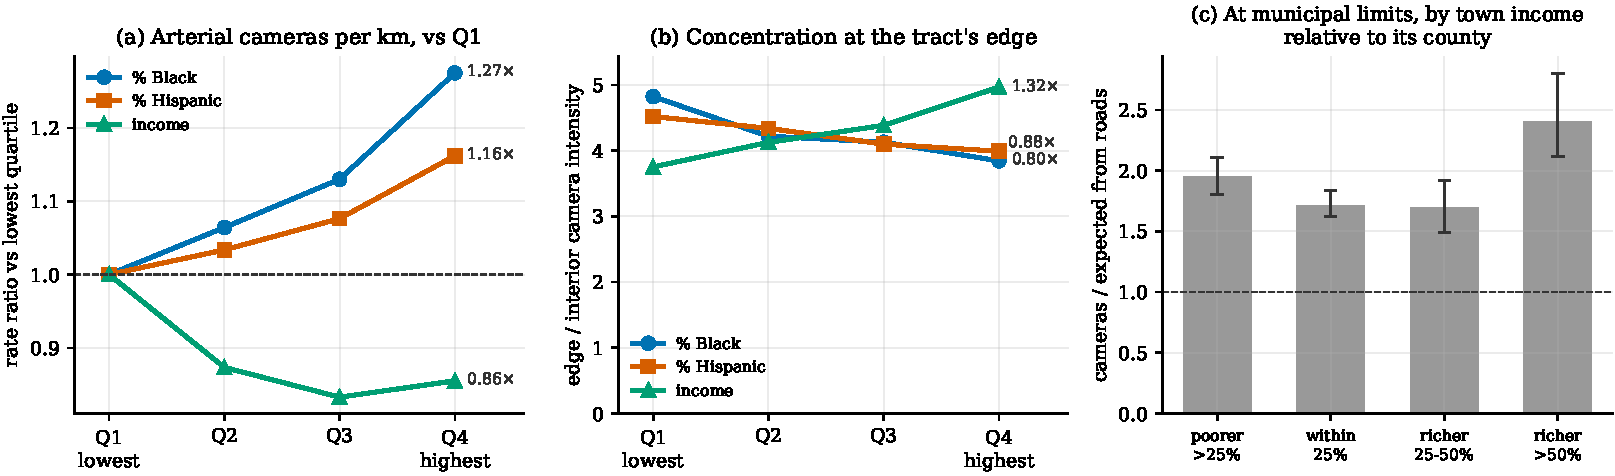
\includegraphics[width=\linewidth]{figures/fig_siting.pdf}
\caption{(a) Arterial cameras per kilometre of arterial road in each quartile relative to the
lowest, ranked within county and density tercile (Mantel--Haenszel), with the Q4/Q1 ratio. (b) Camera intensity within
\SI{50}{\metre} of a tract's boundary over its interior, same ranking: minority tracts' cameras
stand relatively inside them, wealthy tracts' at their edges. (c) Cameras within
\SI{50}{\metre} of an incorporated municipality's limits over the number expected from roads of
the same class in the same county, by the town's median income relative to its county's.}
\label{fig:siting}
\end{figure}

\paragraph{Cameras stand more densely inside Black and Hispanic neighbourhoods, even within a
county.} Per kilometre of arterial road, tracts in the highest quartile of Black population carry
\num{1.74}$\times$ [1.59--1.92] the cameras of the lowest quartile in the same county, and
\num{1.27}$\times$ [1.19--1.36] compared only with tracts of similar density there
(\Cref{tab:siting}, \Cref{fig:siting}a); on residential streets \num{1.59}$\times$ [1.41--1.81];
for cameras whose operator is tagged as a police department \num{1.87}$\times$ [1.52--2.30]. The
Hispanic gradients are smaller but of the same kind (\numrange{1.16}{1.27}$\times$), block groups
reproduce the arterial and residential ones, and so does the plainest comparison available:
majority-Black tracts against majority-white tracts of the same county, in the 542 counties that
have both, carry \num{1.20}$\times$ [1.03--1.41] the cameras per kilometre of road, and
majority-Hispanic tracts, in the 355 counties that have both, \num{1.33}$\times$
[1.12--1.66]. Unlike the commute-exposure contrasts of
\Cref{sec:results:trend}, these did not move with the map. On the maps of July 2025, January 2026, July 2026 and September
2026 the within-county Black gradient in cameras per kilometre of road was \num{1.96}, \num{1.89},
\num{1.83} and \num{1.83} (\num{1.50}, \num{1.45}, \num{1.41} and \num{1.41} within county and density
band) while the map grew six-fold. A pattern produced by where
volunteers happened to map first would have shifted as the map filled in; this one held.

\paragraph{Nor do they simply follow the traffic.} Cameras do follow traffic. Per kilometre, a
surface road carrying \numrange{10000}{20000} vehicles a day has 32 times the cameras of one
carrying fewer than \num{2000}; per vehicle-kilometre it has \num{1.7} times as many. But the
roads of Black and Hispanic neighbourhoods are only slightly busier than the same class of road
elsewhere in their county: in the most-Black tracts they carry \SI{4}{\percent} [2--5] more
traffic per kilometre than in the least-Black tracts of the same county and density band.
Compared class by class on the counted network, cameras stand \num{1.24}$\times$ [1.16--1.33] as
densely per kilometre in the most-Black tracts and \num{1.20}$\times$ [1.13--1.28] per
vehicle-kilometre; per vehicle-kilometre, \num{1.10}$\times$ [1.04--1.18] in the most-Hispanic
and \num{0.82}$\times$ [0.76--0.89] in the richest (\Cref{tab:siting}). Police-operated cameras on
surface roads stand \num{1.72}$\times$ [1.38--2.10] as densely per vehicle-kilometre in the
most-Black tracts. Block groups agree, and so does a \SI{50}{\metre} rule for which road a camera
watches. One comparison does shrink the gradient, and it is instructive. Pooling every counted
road without comparing like with like gives \num{1.09}$\times$ [1.03--1.16] by Black share and
\num{1.00}$\times$ [0.94--1.08] by Hispanic share, because freeways carry \SI{43}{\percent} of the
counted traffic but only \SI{7}{\percent} of the cameras on counted roads, and they make up \num{1.40}$\times$
[1.34--1.47] as large a share of the counted network, and \num{1.15}$\times$ [1.11--1.18] as
large a share of its traffic, in the most-Black tracts as in the least-Black of the same county
and density band, a legacy of routing Interstates through Black
neighbourhoods \citep{archer2020}. Charged to those tracts, through traffic that cameras seldom
watch dilutes their rate for a reason unrelated to where cameras are put.

\paragraph{The cordon reading is not supported.} If cameras watched the entrances and exits of
minority neighbourhoods, those neighbourhoods' cameras would concentrate at their edges. They do
the opposite. Relative to their interiors, the edges of the most-Black tracts carry
\num{0.80}$\times$ [0.75--0.84] the concentration found at the edges of the least-Black tracts
in the same county and density band, and the most-Hispanic \num{0.88}$\times$ [0.82--0.94]
(\Cref{fig:siting}b): a minority neighbourhood's cameras stand inside it. Boundaries in general
attract cameras---within \SI{50}{\metre} of a tract boundary they are \num{1.39}$\times$
[1.35--1.44] as frequent as on roads of the same class in the same county---and boundaries
between racially different neighbourhoods slightly more: at block-group seams where the Black
share differs by ten points or more, cameras are \SIrange{10}{16}{\percent} over-represented. But
at seams where it differs by thirty points or more they show no preference for either side, in where they stand (\num{1.01}$\times$
[0.98--1.04] on the higher-Black side) or in which way they face (\SI{50.7}{\percent} into it).

\paragraph{The protection reading is contradicted within counties; the perimeter pattern belongs
to the wealthy.} Between counties, wealthier tracts do have more cameras---about twice as many
per kilometre of road nationally, the purchasing pattern of richer jurisdictions. Within a
county the richest quartile has \num{0.65}$\times$ [0.58--0.71] the arterial cameras per
kilometre of the poorest, \num{0.86}$\times$ [0.79--0.92] once density is held fixed, and
\num{0.57}$\times$ [0.47--0.69] the police-operated cameras once density is held fixed
(\num{0.40}$\times$ within county alone). What wealth predicts is where a
neighbourhood's cameras stand: the richest tracts' residential-street cameras are
\num{2.43}$\times$ [2.05--2.86] as concentrated at the tract's edge as the poorest tracts'. (The
930 cameras tagged as watching an entrance or gate, or operated by a homeowners' association, are
too few to say whether they lean rich: \num{1.37}$\times$ [0.95--1.99].) At the scale of municipalities
the pattern is plainer (\Cref{fig:siting}c). Within \SI{50}{\metre} of an incorporated
city's limits, cameras are \num{1.81}$\times$ [1.72--1.91] as frequent as on roads of the same class
in the same county. The concentration is greatest around towns more than half again as rich as
their county (\num{2.41}$\times$ [2.12--2.80]), where \SI{86}{\percent} of the limit cameras stand
just inside the town, though towns more than a quarter poorer than their county ring their
limits too (\num{1.95}$\times$ [1.80--2.11]). Where the cameras point adds little to where they stand: of the
heads that look across a limit, the share looking in from outside exceeds the share of cameras
standing outside by six to eight points in every income group. Atlantic City's evaluated deployment, with fixed readers on all
entrances and exits to the city \citep{shjarback2025}, is the policy these numbers
describe.

\paragraph{Why commute exposure hides it.} These gradients are local, and a commute is not---the
uncertain geographic context problem of \citet{kwan2012} in miniature. Of the
cameras a commute passes, \SI{80}{\percent} are more than \SI{2}{\kilo\metre} from both its ends,
and the home tract with its edge accounts for \SI{6.5}{\percent}. Within their county, residents
of the most-Black tracts pass \num{1.28}$\times$ [1.15--1.43] as many cameras in the ring within
\SI{2}{\kilo\metre} of home as residents of the least-Black tracts (\num{1.17}$\times$ within
county and density band), residents of the most-Hispanic tracts \num{1.31}$\times$, and residents
of the richest tracts \num{0.67}$\times$ [0.60--0.75] as many as the poorest's; over a whole
commute these dilute to \num{1.06}$\times$, \num{1.00}$\times$ and \num{0.94}$\times$. The
conclusion of \Cref{sec:results:coverage} stands for what it measured: within a county, the
burden of passing cameras on the way to work is close to equal. Where the cameras are placed is
not.

\paragraph{What this cannot show.} Traffic is counted only on the federal-aid network, so
residential streets are still compared per kilometre, and on many sections the count is an
estimate factored from a short or earlier count rather than a continuous measurement. Nor can
siting data separate motive from rationale. Police departments cite crime, and sometimes
traffic, when asked why cameras stand where they do \citep{musgrave2023,witte2026}, and neither
is spread evenly across neighbourhoods; the gradients are disparities in where surveillance is
sited, not findings about intent. Business-operated cameras, nearly nine in ten of them Lowe's or
The Home Depot's, show an even steeper racial gradient (\num{2.24}$\times$ [1.81--2.77]), a
reminder that land use shapes siting as well as policing does. And within-county gradients could
still reflect mapping that is uneven inside cities: their stability across four maps argues
against a transient artefact of mapping progress, not against a persistent one. What can be
checked is coverage between cities. Against Flock Safety's own transparency portals the map
holds, at the median, \num{0.98} of the cameras that \num{1050} municipal police departments
report operating (\num{28349} mapped inside their limits against \num{31210} reported), and how
completely a city is mapped is unrelated to its Black share (Spearman $\rho=0.06$ [$-0.003$,
$0.12$]) and only weakly related to its Hispanic share ($\rho=0.085$ [0.025, 0.14]) and its
income ($\rho=0.12$ [0.06, 0.18]); the strongest predictor is size, small towns being the least
completely mapped ($\rho=0.39$) \citep{eyesonflock}. Those are the cities that publish counts.
Against national totals the map is less complete: Flock has said it operates more than
\num{120000} cameras nationwide, and a researcher's map built from its records in December 2025
shows more than \num{170000} cameras of all kinds \citep{mazurov2026}, against the \num{114352} Flock cameras on our map in the
fifty states and DC. Coverage outside the portal cities, and of cameras no department reports,
is the larger unknown.
In the one region with an authoritative list---the locations of 614 Flock cameras in Hampton
Roads, Virginia, unsealed by a federal court in 2025---a study built on that list found
majority-Black tracts carrying about four times the cameras of majority-white
ones \citep{keener2026}; on our map the same comparison gives
\num{1.8} times per tract. Our map holds nearly twice as many cameras there as the police list,
including other owners', which would dilute a police-driven gradient---as the steeper gradient of
police-operated cameras nationally suggests it does.

\subsection{Thirty-three months of mapping}
\label{sec:results:trend}

Everything above describes the map of 22 September 2026. We re-asked the same questions of
the map as it stood on five earlier dates, reconstructed exactly from OpenStreetMap's
history (\Cref{sec:data:history}), and of the July 2026 snapshot: the same \num{56131}
commutes on the same roads, each saved route re-scored against each date's cones, and every
commute that passed a camera on a date routed again to avoid that date's cameras
(\Cref{sec:method:history}; the July snapshot was re-scored only). \Cref{tab:trend} and
\Cref{fig:trend} give the national picture, \Cref{fig:trend_states} every state. Each date
should be read as what had been \emph{mapped} by then, not what had been installed.

\begin{table}[tbp]
\centering
\small
\caption{The same \num{56131} commutes on the same roads against the camera map of each
date, commuter-weighted. Exposure from re-scoring each saved route; avoidance from routing
every commute exposed on that date, with the share reaching zero and the median extra time
given for those commuters. The July 2026 snapshot was re-scored, not re-routed.}
\label{tab:trend}
% generated by make_tables.py
\begin{tabular}{lrrrrrrr}
\toprule
Map date & Mapped & \multicolumn{2}{c}{Passing $\geq$1 (\%)} & Mean & Exposed who & Extra min, & Min per \\
& ALPR & & [95\% CI] & passed & reach zero (\%) & exposed & camera \\
\midrule
2024-01-01 & \num{1112} & \num{2.2} & [2.0--2.4] & \num{0.05} & \num{95.0} & \num{0.77} & \num{0.42} \\
2024-04-01 & \num{1267} & \num{2.9} & [2.7--3.1] & \num{0.08} & \num{95.7} & \num{1.04} & \num{0.51} \\
2024-07-01 & \num{1420} & \num{3.3} & [3.0--3.5] & \num{0.08} & \num{96.0} & \num{1.00} & \num{0.49} \\
2024-10-01 & \num{1581} & \num{3.5} & [3.2--3.7] & \num{0.09} & \num{96.0} & \num{1.02} & \num{0.52} \\
2025-01-01 & \num{7583} & \num{12.3} & [11.9--12.7] & \num{0.35} & \num{92.5} & \num{1.20} & \num{0.61} \\
2025-04-01 & \num{14238} & \num{20.4} & [19.9--20.9] & \num{0.59} & \num{92.7} & \num{1.24} & \num{0.63} \\
2025-07-01 & \num{22690} & \num{29.4} & [28.8--30.0] & \num{0.94} & \num{92.4} & \num{1.36} & \num{0.65} \\
2025-10-01 & \num{34383} & \num{38.4} & [37.8--39.0] & \num{1.33} & \num{91.6} & \num{1.51} & \num{0.66} \\
2026-01-01 & \num{63522} & \num{55.9} & [55.3--56.4] & \num{2.44} & \num{86.9} & \num{1.98} & \num{0.70} \\
2026-04-01 & \num{85845} & \num{63.4} & [62.8--63.9] & \num{3.14} & \num{84.7} & \num{2.32} & \num{0.73} \\
2026-07-01 & \num{109853} & \num{69.6} & [69.1--70.1] & \num{4.08} & \num{82.6} & \num{2.67} & \num{0.75} \\
2026-09-22 & \num{142257} & \num{75.3} & [74.8--75.7] & \num{5.14} & \num{79.0} & \num{3.14} & \num{0.76} \\
\midrule
\quad + registry & \num{186316} & \num{78.6} & [78.1--79.0] & \num{6.24} & \num{75.5} & \num{3.92} & \num{0.83} \\
\bottomrule
\end{tabular}

\end{table}

\begin{figure}[tbp]
\centering
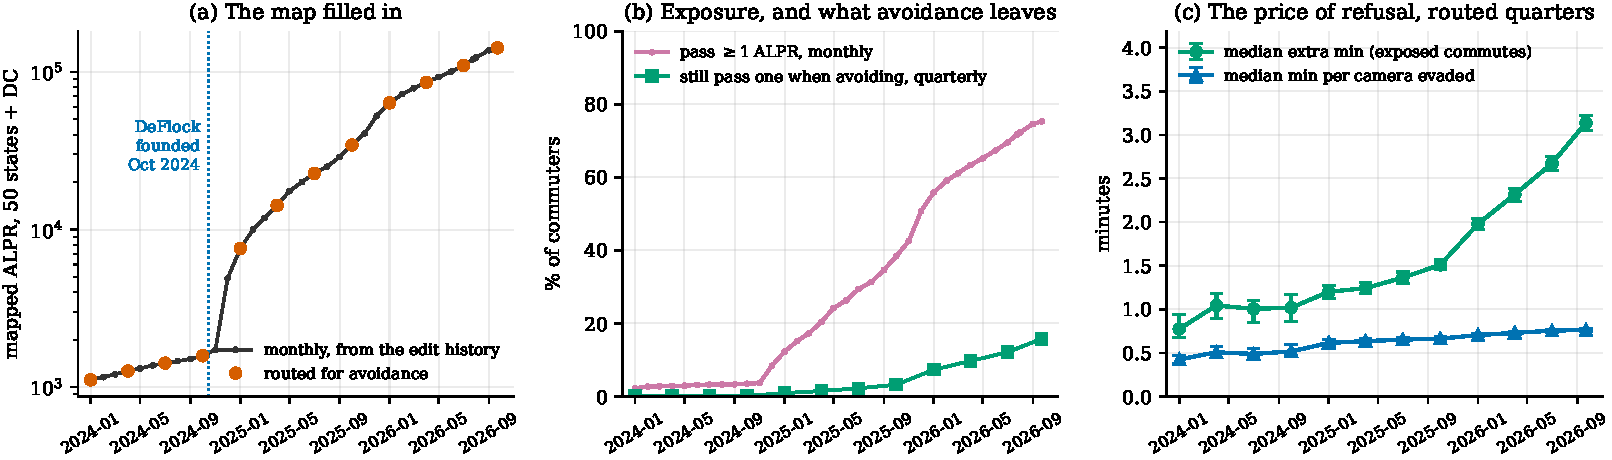
\includegraphics[width=\linewidth]{figures/fig_trend.pdf}
\caption{(a) Mapped \alpr in the fifty states and DC: monthly from the ohsome history API,
and the study's seven maps. (b) Share of commuters passing at least one mapped reader
(\SI{95}{\percent} CIs), and the share still passing one on the avoiding route. (c) For
commuters exposed on each date, the median extra minutes to avoid every camera, and the
median minutes per camera evaded.}
\label{fig:trend}
\end{figure}

\paragraph{The map filled in.} On 1 January 2024 OpenStreetMap held \num{1112} \alpr
installations in the fifty states and the District of Columbia, four-fifths of them with no
vendor tag, and twenty-six jurisdictions had none at all. Growth was slow until DeFlock was
founded in October 2024 and abrupt after it: \num{7583} by January 2025, \num{22690} by
July, \num{63522} by January 2026 and \num{142257} by September, a 128-fold increase in
thirty-three months (\Cref{fig:trend}a). By July 2025 only Hawaii, Vermont and Alaska had
none; by September 2026 every state had some. Flock's share of the mapped network went from
\SI{17}{\percent} to \SI{72}{\percent} during 2024 and has stayed near four-fifths since,
while the untagged share fell from \SI{81}{\percent} to \SI{5}{\percent} and the named
non-Flock vendors rose from \SI{1}{\percent} to \SI{15}{\percent} as contributors tagged them.

\paragraph{Exposure followed the map, almost in proportion.} The share of commuters passing
at least one mapped reader went from \SI{2.2}{\percent} to \SI{12.3}{\percent},
\SI{29.4}{\percent}, \SI{55.9}{\percent} and \SI{75.3}{\percent}; the mean from \num{0.05}
cameras to \num{5.14}. Against the number of mapped cameras the elasticity is \num{0.92}
across the seven maps. Per camera mapped, exposure has fallen by about a quarter since
January 2024, from \num{0.049} to \num{0.036} encounters per commute per thousand cameras:
the cameras mapped later lie on commute routes slightly less often than those mapped first,
but not much less. Nor is there a sign of saturation. The last two months alone brought
\SI{18.3}{\percent} more mapped cameras and \SI{17.0}{\percent} more encounters.

\begin{figure}[tbp]
\centering
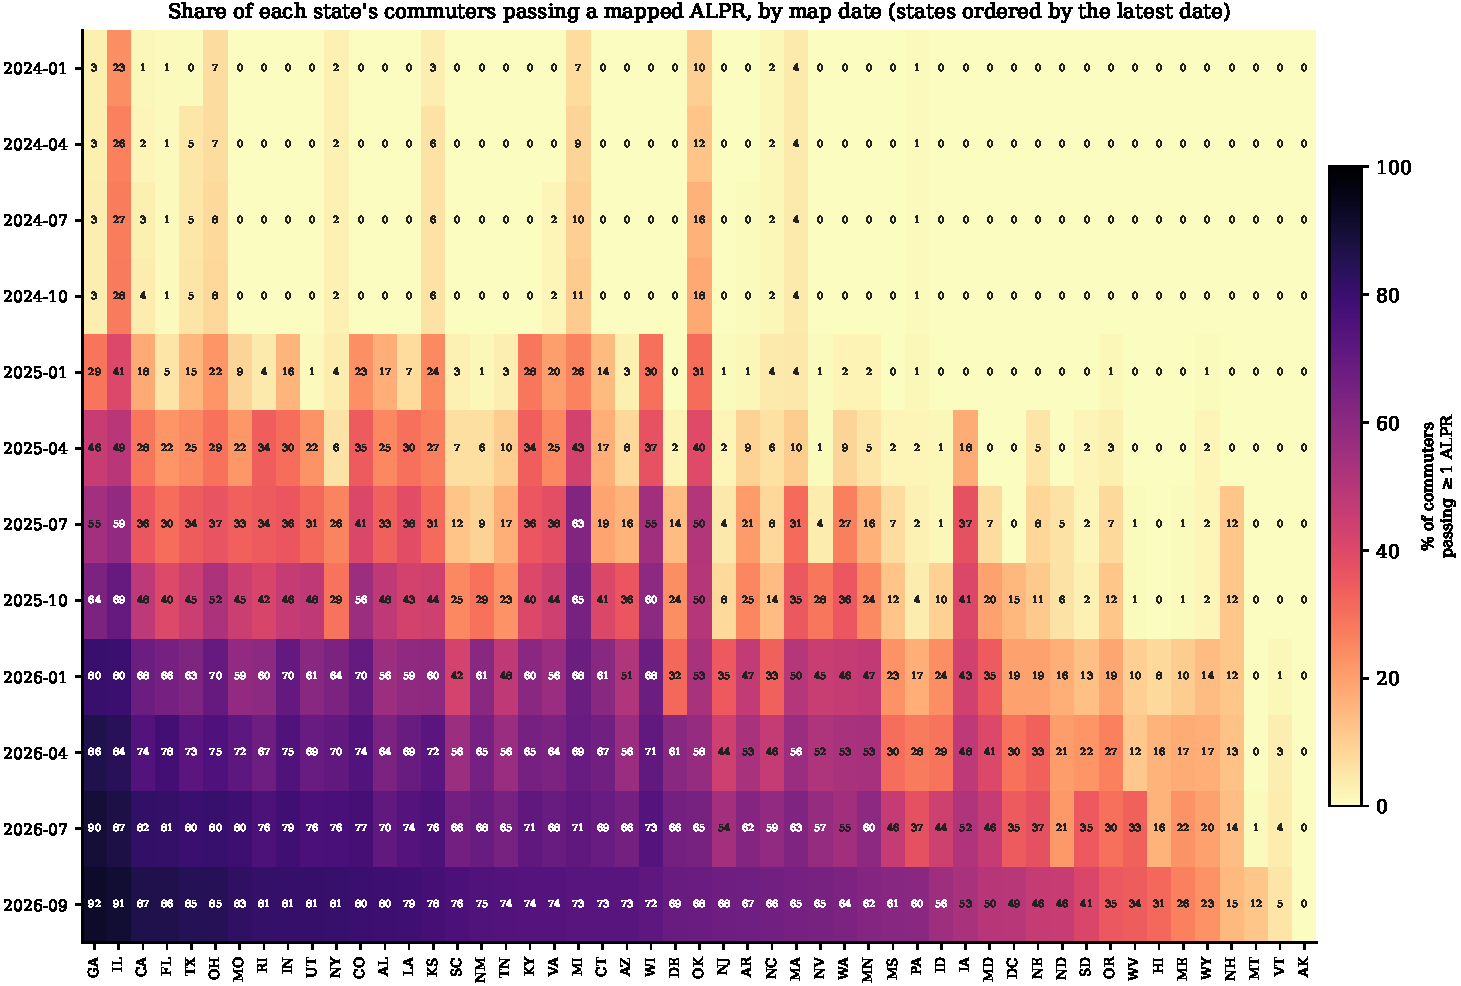
\includegraphics[width=\linewidth]{figures/fig_trend_states.pdf}
\caption{Share of each state's commuters passing at least one mapped \alpr on each map,
states ordered by the latest.}
\label{fig:trend_states}
\end{figure}

\paragraph{The states filled in at different times.} In January 2024 Illinois was the only
state where more than a tenth of commuters passed a mapped reader (\SI{23.5}{\percent}); by
January 2025 fifteen were, by July 2025 thirty-one, by January 2026 forty-seven
(\Cref{fig:trend_states}). In July 2025 Michigan's commuters were the most exposed of any
state's (\SI{62.8}{\percent}), while Pennsylvania (\SI{2.4}{\percent}), Nevada
(\SI{3.8}{\percent}), New Jersey (\SI{4.4}{\percent}) and North Carolina (\SI{8.2}{\percent})
would have looked nearly camera-free; all four are between \SI{60}{\percent} and
\SI{68}{\percent} today. A state's rank on the January 2025 map predicts its rank today only
moderately (Spearman $\rho=0.80$ on mean exposure; from January 2024, $0.54$). Nor does the
map only grow. Wisconsin and Iowa each gained cameras on net between July and September 2026
yet lost about three points of exposure: 190 and 123 of their July cameras left the map,
deleted or retagged, and the cameras newly mapped added less exposure than was lost.

\paragraph{Refusal got dearer, and not only because there was more to refuse.} On the
sparse maps of 2024 a commuter who passed a mapped camera could almost always get around it:
\SI{95.0}{\percent} [92.7--96.9] of exposed commuters could reach zero, for a median of
\SI{0.77}{\minute}. On the September 2026 map \SI{79.0}{\percent} [78.4--79.7] can, for a
median of \SI{3.14}{\minute}, having declined on every map since mid-2024 (\Cref{tab:trend};
\Cref{fig:trend}c). Most of that rise is the number of cameras on each trip, but the price of
evading each one rose too, from \SI{0.42}{\minute} [0.38--0.47] to \SI{0.76}{\minute}
[0.75--0.78]. Two things moved it, and a fixed sample can separate them. One is who was
exposed: the early maps covered dense metropolitan grids, where \Cref{sec:results:geo} finds
evasion cheapest, and the later ones reached rural and intercity roads. The other happened on
the same trips. Followed from the July 2025 map to September 2026's, the \num{12647} commutes
exposed in July came to pass \num{9.9} cameras on average instead of \num{3.2}; the share of
them that can reach zero fell from \SI{92.4}{\percent} to \SI{72.6}{\percent}, and the price
per camera rose from \SI{0.65}{\minute} [0.63--0.68] to \SI{0.81}{\minute} [0.79--0.84].
Every cohort followed for fifteen months or more shows the same---\SIrange{24}{35}{\percent}
more per camera by September 2026, each interval clear of its starting one: as more of a
trip's cameras, and of its alternatives', are mapped, each costs more to avoid. Over the two months between the 2026 snapshots the change is too small to
see, which is why the fifteen-state comparison below finds the price per camera
unchanged.

\begin{figure}[tbp]
\centering
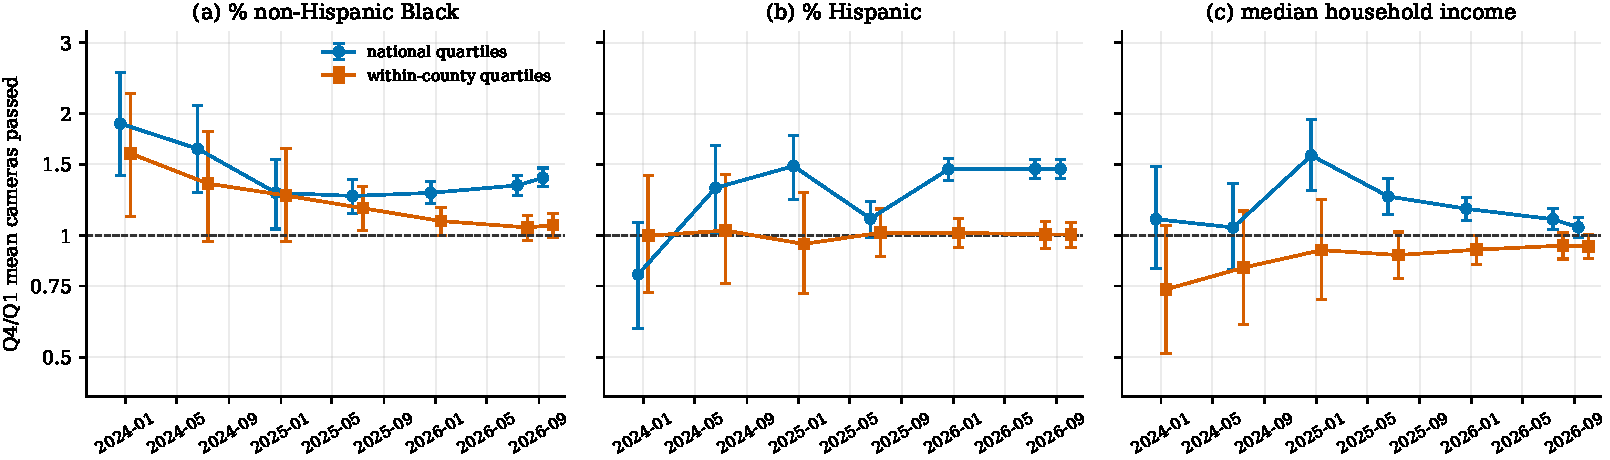
\includegraphics[width=\linewidth]{figures/fig_trend_gradients.pdf}
\caption{The demographic contrasts of \Cref{fig:within} on every map: mean cameras passed
from the highest quartile of origin tracts over the lowest (for income, the richest over the
poorest), with quartiles ranked nationally and within county, and \SI{95}{\percent} CIs on
the ratio from the commute-level bootstrap; resampling counties widens them, about twofold on the
early maps (\Cref{sec:results:trend}). Log scale; the dashed line is parity.}
\label{fig:trend_gradients}
\end{figure}

\paragraph{The national equity gradients moved with the map.} \Cref{fig:trend_gradients}
repeats the contrasts of \Cref{sec:results:demo,sec:results:coverage} on every map. A study
run on the January 2025 map would have reported that commuters from the richest quartile of
tracts pass \num{1.58}$\times$ [1.30--1.93] as many cameras as those from the poorest; today
the ratio is \num{1.05}$\times$ [0.99--1.11]. The Hispanic contrast was \num{0.80}$\times$
[0.59--1.08] in January 2024, \num{1.48}$\times$ [1.22--1.77] a year later,
\num{1.10}$\times$ [0.99--1.21] in July 2025, and \num{1.46}$\times$ from January 2026 on.
Each would have been reported with a confidence interval, three of the six quoted here
excluding parity under either bootstrap, and each describes at least in part where contributors
had reached. Ranked
within county, the Hispanic contrast lies between \num{0.95} and \num{1.03} on every map, and
the income contrast between \num{0.74} and \num{0.94}---at or below parity---on every map.

The Black contrast is the instructive exception. Nationally it fell from \num{1.89}$\times$
to \num{1.25}$\times$ by July 2025 and has risen since, to \num{1.39}$\times$. Within
counties it was \num{1.60}$\times$ [1.12--2.24] on the January 2024 map---\num{1112}
cameras, four-fifths without a vendor tag, past which \SI{2.2}{\percent} of commuters
drove---and it has fallen steadily since: \num{1.34} and \num{1.26} on the next two maps,
\num{1.17} [1.03--1.32] in July 2025, \num{1.09} in January 2026, and \num{1.05} and
\num{1.06} [0.99--1.13] on the two 2026 snapshots. Even the early gradients were fragile:
their intervals exclude parity when commutes are resampled, but not when counties are, which on
a sparse map means resampling the few counties whose cameras had been mapped (January 2024
[0.69--2.09], July 2025 [0.99--1.37]). With counties resampled, no within-county contrast clears
parity on any of the six maps so tested; on the seventh, the re-scored July 2026 snapshot, none
clears it even with commutes resampled. On a sparse map the within-county control is not enough. It removes differences in mapping effort between
counties, but when a county's map holds a handful of cameras, which of its neighbourhoods
they stand in is itself the choice of a few contributors, or reflects the few agencies whose
cameras were mapped first. The check we recommend is therefore necessary rather than
sufficient: it becomes informative as the map within counties approaches completeness, and
the convergence toward parity across seven maps is the best evidence available that the
current map is nearer that point than any earlier one.

\paragraph{Fifteen states, fully re-routed.} The trend's last step can be checked against a
comparison that re-routed everything. For the fifteen states of the study's earlier rounds,
the same \num{17580} commutes were routed in full against both 2026 snapshots on the same
road extract, and every baseline route was identical to the metre and the second. Camera
encounters grew by \SI{18.3}{\percent} against \SI{18.7}{\percent} more mapped cameras in those states, the
median price of evading one stayed at \SI{0.78}{\minute} to the second decimal, and
Pennsylvania's mean exposure rose \SI{88}{\percent} in two months.

\paragraph{What follows.} Three things. The absolute exposure figures of this paper are a
lower bound that has risen with every map and will keep rising; any study built on
crowdsourced surveillance data dates, and should say when its map was drawn. The price of
refusal dates as well: it has risen with every map, per camera as well as in total, and
today's figures describe a map that is still filling in. And no
national gradient in commute exposure measured from these data is a finding about cameras
until it has survived both the within-county control and the question of how complete the map
was when it was measured. Over thirty-three months the national exposure gradients rose, fell
and changed direction, while the within-county ones held at parity or converged toward it;
where cameras stand within counties, by contrast, barely moved (\Cref{sec:results:siting}).

\section{Discussion}
\label{sec:discussion}

\subsection{Refusal is cheap, and that is the policy-relevant fact}

The strongest result here is also the simplest: \SI{84.2}{\percent} of American commuters
can reach work past no mapped licence-plate reader, and the avoiding route is a median of
\SI{1.62}{\minute} longer---\SI{3.14}{\minute} for commuters with a camera to avoid. A common
intuition about these networks is that they are, or soon will be, comprehensive enough that
avoidance is futile, so that the privacy loss is unavoidable rather than chosen. At current
mapped density that is false for five commuters in six. It has been false on every map since 2024, but it is
becoming less so: as the map filled in, the share of exposed commuters who can reach zero
fell from \SI{95}{\percent} to \SI{79}{\percent}, and the median cost for those with a camera
to avoid quadrupled (\Cref{sec:results:trend}). Nor, within a county, is the price set by who
lives where: nationally, commuters from the most-Black and most-Hispanic tracts pay more in total
because they pass more cameras, but within their county they pay what their neighbours pay
(\Cref{sec:results:coverage}).

The corollary cuts the other way. If avoidance is this cheap, it is also cheap for people
with reason to evade legitimate investigation, which bounds how much investigative value a
fixed-camera network can deliver against a motivated subject while it continues to read
every unmotivated one.

\subsection{Exposure and siting answer the equity question differently}

We set out to measure whether surveillance burden falls unevenly, and the answer depends on
which burden is meant. Measured as what a commuter passes on the way to work, the national
gradients are real in the data, substantial (\num{1.39}$\times$ by Black and
\num{1.46}$\times$ by Hispanic share of the origin tract) and statistically clean---and they
evaporate under a control any careful reviewer would demand. Measured as where cameras stand, a
within-county gradient survives every control we applied: per kilometre of the same class of
road in the same county and density band, \numrange{1.27}{1.59}$\times$ in the most-Black
tracts, and \num{1.87}$\times$ per kilometre of road for police-operated cameras;
\num{1.20}$\times$ per vehicle-kilometre of counted traffic, so not an artefact of busier roads; stable across four maps; robust to
the thresholds that define it; and in the same direction as the one study built on an
authoritative list of locations \citep{keener2026}. The two are reconciled by distance. The
siting gradient is local, and four-fifths of the cameras a commute passes lie far from either
end, on corridors that everyone in a county drives. A resident of a heavily Black neighbourhood
passes about as many cameras on the way to work as a resident of a white one in the same
county, and lives among more of them.

The map's own history shows why the exposure contrasts need that control. Run on the map of
January 2025, this study would have found that the richest quartile of tracts passes
\num{1.58}$\times$ as many cameras as the poorest; run six months later, that the Hispanic
gradient had shrunk to \num{1.10}$\times$ from \num{1.48}$\times$; run today, that there is
no income gradient and that the Hispanic one is back at \num{1.46}$\times$. Each answer would
have carried a clean confidence interval, and each was a photograph of a mapping effort in
progress (\Cref{sec:results:trend}). The within-county siting gradient, by contrast, barely
moved over the fifteen months for which we could compute it.

We think this generalises. A considerable amount of accessible research on surveillance
infrastructure necessarily rests on volunteer-mapped data, because no authoritative national
inventory exists. Such a study should say which burden it measures. A correlation of exposure
reported without a within-locality control risks describing the demography of \emph{mappers}
rather than of the surveilled, and one from a sparse map is at risk even with the control. A
correlation of siting should compare cameras with the roads they could have stood on, not with
area or population alone, and should stratify rather than pool across places: our own first
pass pooled, and overstated the racial and ethnic siting gradients by \SIrange{20}{35}{\percent}. Weighting by
traffic answers the obvious objection, but only like for like: pooled with surface streets, the
freeway traffic that runs through Black neighbourhoods would have hidden most of the gradient
here. Both need the
date of the map and, where the edit history allows, a check of how the result moves as the map
fills in.

\subsection{Attention and exposure are aimed at different infrastructure}

Flock Safety is the name in municipal council debates, in local journalism, and in the
activist mapping effort that produced the data underlying this paper. It holds four-fifths
of mapped installations. Yet per unit deployed its cameras generate fewer than half as many
camera encounters as other vendors', and the racial gradient in its exposure is weaker
(\num{1.34}$\times$ against \num{1.57}$\times$).

We do not read this as exonerating, for a reason the measurement itself makes clear. A
camera at the entrance of a residential subdivision does something qualitatively different
from a multi-head unit over a six-lane arterial: it observes a small population repeatedly rather than a
large population once, and repeated observation of a known small set is precisely what
makes pattern-of-life inference possible. Commute exposure measures breadth, not depth, and
Flock's model appears optimised for depth. A study designed around repeat observation of
the same vehicle would likely reverse the ordering reported here, and we would expect it
to.

What the result does establish is that, in exposure, a distributional concern has been
attached disproportionately to one vendor: the steeper exposure gradient belongs to other
vendors' cameras, bought, where the operator is known, mostly by police departments too, but
standing more often beside
the arterials and freeways that commuters share---some of them laid through Black
neighbourhoods decades before \alpr existed. Siting tells the other half. Within
counties and density bands, Flock's cameras stand \num{1.42}$\times$ as densely per kilometre
in the most-Black tracts as in the least-Black, and other named vendors' \num{1.44}$\times$: in
where cameras are placed, the vendor in the news is no exception. Regulation aimed only at
Flock would leave the steeper exposure gradient untouched; regulation that exempted it would
leave most of the siting disparity in place.

\subsection{Where the burden actually concentrates}

The distributional finding that rests least on the map is geographic rather than
demographic, and it is counter-intuitive: per camera, avoidance tends to be cheapest in dense
metropolitan grids and dearest in rural and intercity travel. Network topology, not camera
count alone, sets the price of refusal. The tendency is modest across whole states
(\Cref{sec:results:geo}), but it rests on road-network structure---which OSM maps close to
completely---rather than on camera counts, so it is robust to the coverage critique in a way no
result built on counts can fully be, however well checked.

\section{Limitations}
\label{sec:limitations}

\subsection{Tract centroids are not addresses}

Every route runs centroid to centroid; real commutes begin in a driveway. In large or
irregular tracts the centroid can sit far from any residence. This adds noise in both
directions and is the main reason we report distributions rather than point estimates. It
also costs coverage: where a tract's internal point lies too far from any road to snap to,
the commute cannot be routed at all, which removes a fifth or more of the sample in Alaska,
Hawaii, Montana and Wyoming (\Cref{sec:method:exec}).

The stricter caution: tract demographics describe tracts, not the people routed.
``Commutes originating in high-poverty tracts pass more cameras'' is supportable; ``poor
people pass more cameras'' is not---the ecological fallacy of \citet{robinson1950}. Results can
also depend on the areal unit \citep{openshaw1984}, which is why the siting analysis is repeated
at block-group scale.

\subsection{Crowdsourced camera data is non-randomly missing}
\label{sec:coverage}

Absolute exposure figures are a \textbf{lower bound}: like volunteered geographic data
generally \citep{haklay2010,herfort2023}, the map is least complete where contributors are
absent, and there cameras are missing from the map but present on the pole. The hazard is not
undercounting but its correlation with the variables of interest, quantified in
\Cref{sec:results:coverage}. Where police departments publish counts, the map is close to
complete and its completeness is unrelated to a city's Black share (\Cref{sec:results:siting});
nationally, by Flock's own statement and a researcher's map of its records, it holds at most
\SI{95}{\percent}, and perhaps two-thirds, of Flock's cameras \citep{mazurov2026}, and how the missing ones are distributed is
unknown. Every demographic statement in this paper is conditional on that, and the condition is
not a formality.

\subsection{Cone geometry: swept, and one result depends on it}
\label{sec:lim:geom}

The \SI{60}{\metre} radius was chosen by reasoning---a pole set back from the kerb needs a
cone long enough to reach the carriageway it watches---and the \ang{45} default span from
the \SI{82}{\percent} of explicit arcs that span exactly that. Neither was measured. We
therefore swept the radius over $\{30, 45, 60, 90\}\,\si{\metre}$, rebuilding the cone
geometry at each and re-scoring all \num{56131} routes (\Cref{fig:radius}).

\begin{table}[htbp]
\centering
\small
\caption{Cone-radius sensitivity, commuter-weighted. Exposure is mildly sensitive to the
assumption; the avoidance result is not, until the radius grows by half. At the assumed
\SI{60}{\metre} the clean share is \SI{83.7}{\percent} rather than the \SI{84.2}{\percent}
of \Cref{tab:headline} because the sweep re-scores stored route geometry
(\Cref{sec:method:history}).}
\label{tab:radius}
\begin{tabular}{lrrrr}
\toprule
Radius & Mean cameras & vs \SI{60}{\metre} & Avoided routes still clean & Residual \\
\midrule
\SI{30}{\metre} & \num{3.82} & \num{0.74}$\times$ & \SI{87.4}{\percent} & \SI{5.4}{\percent} \\
\SI{45}{\metre} & \num{4.62} & \num{0.90}$\times$ & \SI{85.6}{\percent} & \SI{5.2}{\percent} \\
\SI{60}{\metre} & \num{5.14} & assumed            & \SI{83.7}{\percent} & \SI{5.3}{\percent} \\
\SI{90}{\metre} & \num{5.88} & \num{1.14}$\times$ & \textbf{\SI{55.1}{\percent}} & \SI{21.7}{\percent} \\
\bottomrule
\end{tabular}
\end{table}

\begin{figure}[tbp]
\centering
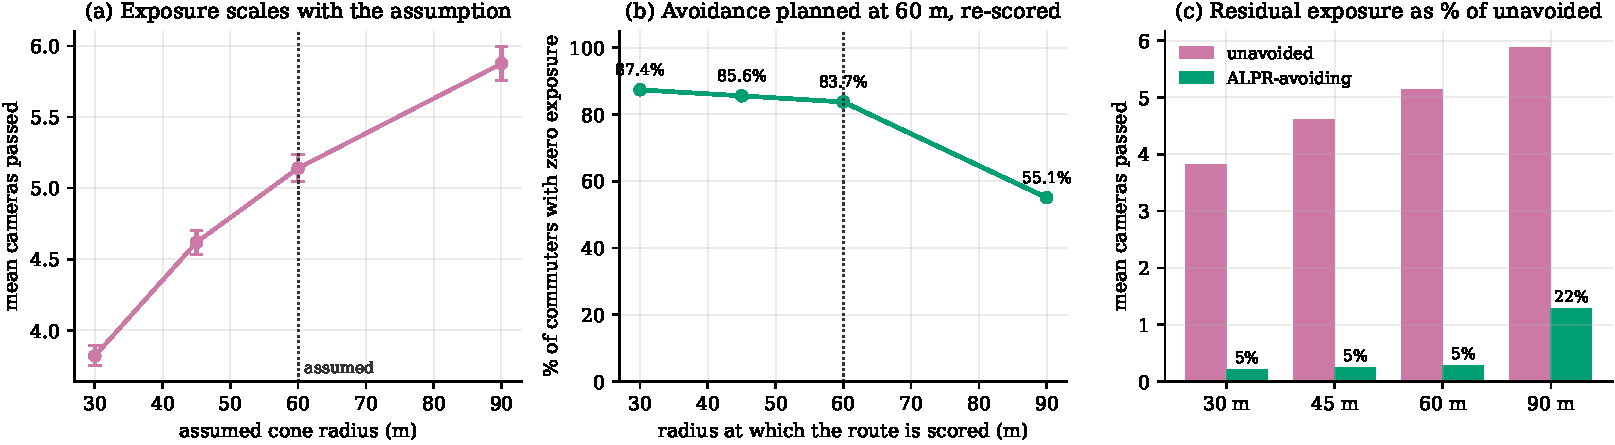
\includegraphics[width=\linewidth]{figures/fig_radius.pdf}
\caption{Sensitivity to the assumed cone radius. (a) Measured exposure scales gently---
halving the radius removes only a quarter of it. (b) The share of commuters reaching zero
exposure is flat below the assumed value and falls sharply above it. (c) Residual exposure
as a fraction of unavoided, by radius.}
\label{fig:radius}
\end{figure}

Two things follow, and they point in opposite directions.

\textbf{Exposure is robust.} Halving the radius removes only a quarter of the measured
exposure, and \SI{90}{\metre} adds \SI{14}{\percent}. Cones are small relative to the road
network at any of these values, so \Cref{sec:results:exposure} does not rest on the choice.

\textbf{The avoidance headline does depend on it.} Routes planned against \SI{60}{\metre}
cones remain clean when re-scored at \SI{45}{\metre} and \SI{30}{\metre}---avoidance is not
finely tuned to the assumption from below. But at \SI{90}{\metre} the share reaching zero
falls from \SI{83.7}{\percent} to \SI{55.1}{\percent}, a drop of \num{28.7} points
(\SI{95}{\percent} CI $[-29.3, -28.1]$), and residual exposure quadruples from
\SI{5.3}{\percent} to \SI{21.7}{\percent} of baseline. If real fields of view are half again
as long as we assume, more than a third of the routes this paper counts as clean are not.

That figure is nonetheless a \emph{lower} bound rather than an estimate, for a reason worth
being precise about. These routes were \emph{planned} against \SI{60}{\metre} cones and only
\emph{re-scored} at \SI{90}{\metre}; a router given \SI{90}{\metre} cones would find
different clean routes, and the denser the network the more of them there are. Measuring
the true value requires a complete re-route at each radius---most of a day apiece at this
sample's size---which we have not done. What the sweep establishes is that the
avoidance claim is conditional on the radius in a way the exposure claim is not, and that
the conditionality bites only above the assumed value.

\subsection{A single avoidance strength}

All results use the strongest setting. Intermediate settings are the practically
interesting ones for a shipped application, and in informal tests they behaved badly: the
useful range was roughly $0.3\rightarrow0.01$, and whether a setting took effect depended on
local camera density. On two test routes a setting of \num{0.3} avoided none of six cameras
between Wilmington and Dover, Delaware, and five of eight across metropolitan Atlanta. A single
fixed slider-to-multiplier mapping is therefore unlikely to serve; the mapping may need to
adapt to local density. This is an open problem for the application and an unmeasured
dimension of this paper.

\subsection{Sample scope}

All fifty states and the District of Columbia, but within-state commutes only
(\texttt{od\_main}), so cross-border metropolitan areas---New York/New Jersey,
Philadelphia, Washington, Kansas City, St Louis, Portland---are systematically truncated at
the state line. Several are exactly the dense multi-jurisdiction areas where the question
is most pointed. The District is the extreme case: most people who work there live in
Maryland or Virginia, so its sample describes only commutes with both ends inside the
District. Alaska's flows are from 2016 and Michigan's from 2021, the latest LODES
publishes; the other 49 jurisdictions' are from 2022.

\subsection{Past maps record mapping, not deployment}

The trend of \Cref{sec:results:trend} is a trend in what had been mapped. OpenStreetMap's
installation dates are too sparse to separate the two---47 of \num{142991} nodes carry
one---so a camera first mapped in 2026 may have stood since 2021, and the 128-fold growth of
the map cannot be read as a rate of deployment. Absolute figures date accordingly. The
relative claims are the ones to carry forward, and across seven maps they held: the
cheapness of refusal---under a minute per camera evaded on every map, though rising---the
within-county collapse of the national exposure gradients on the 2026 maps, and their
convergence toward it before, the instability of the national exposure gradients themselves, and, on the four maps
tested, the stability of the within-county siting gradient. What the maps cannot establish is that
the current one is complete. The convergence of the within-county ratios toward parity is
what a true effect of zero would produce, and also what a real effect would produce if it
were concentrated in counties still being mapped. The other vendors' within-county gradient
of \Cref{sec:results:vendor}---distinguishable across the fifteen states of the September round,
on the line across all fifty-one---is where that distinction matters most, and a
vendor-resolved trend would test it.

\subsection{Free-flow travel times}

Routing uses free-flow speeds with no traffic, time-of-day, or turn-restriction penalties,
so both travel times are optimistic. The \emph{difference} between them---the quantity
actually reported---is more robust than either absolute, since both share the bias.

\subsection{Avoidance is a preference, not a guarantee}

\texttt{multiply\_by: 0.01} makes observed roads expensive, not impassable. Where no
alternative exists the router correctly uses the watched road. ``Zero cameras'' means the
optimiser found a clean path, not that one was guaranteed to exist.

\section{Ethics and dual use}
\label{sec:ethics}

The study uses only public data. The camera locations are volunteers' observations from public
places, already published in OpenStreetMap under an open licence; the commute flows and
neighbourhood attributes are Census Bureau aggregates, published with the Bureau's
confidentiality protections and attached to census tracts rather than to people; the portal
counts are published by the police departments themselves. No individual is identified, no
one's travel was observed, and the paper adds no camera location to the public record.

The routing engine is dual-use, and we weighed that before publishing it. It lets anyone decline
to be photographed on the way to work, including someone with reason to evade a lawful
investigation. Three considerations decided the matter. The capability is not new: the camera
map is public, and several services already route drivers around it
\citep{deflockmaps,flockhopper,banditkin}. The result it rests on bounds the investigative
value of fixed cameras against a motivated subject whether or not the tool exists
(\Cref{sec:discussion}); what such a network reliably records is the unmotivated majority. And
the measurement itself---how much surveillance an ordinary trip passes, what declining it costs,
and near whom the cameras stand---is information a public debate about the technology needs and
has not had. The software is released under GPLv3, and its routing server is not exposed to the
internet by default (\Cref{sec:system}).

\section{Reproducibility}

Code, configuration, and the derived outputs behind every table and figure---per-commute
results, per-state tables, the siting tables and every analysis report quoted in the text---are
in the project repository, \url{https://github.com/KaraZajac/TRAMES}, under
\texttt{research/}. Fixed seed \texttt{20260725} throughout, for both sampling and bootstrap.
All external data sources are public and require no API key. Beyond the routing server, the
analysis needs Python with NumPy, Shapely and Matplotlib; pyosmium for the road sample; and
pyogrio, which bundles GDAL, only to read the HPMS geodatabase.

\begin{table}[htbp]
\centering
\small
\begin{tabular}{ll}
\toprule
Component & Path \\
\midrule
Data acquisition            & \texttt{research/data/fetch.sh} \\
Camera fetch (continental)  & \texttt{server/alpr/fetch-na-cones.sh} \\
Cone construction           & \texttt{server/alpr/build\_cones.py} \\
Past camera maps (Overpass)  & \texttt{server/alpr/fetch-history.sh} \\
Past camera maps (history dump) & \texttt{server/alpr/history\_from\_planet.py} \\
Monthly mapping history     & \texttt{research/scripts/fetch\_mapping\_history.py} \\
Cone-set variants           & \texttt{server/alpr/build-variants.sh} \\
Snapshot statistics         & \texttt{research/scripts/snapshot\_stats.py} \\
Routing configuration       & \texttt{server/graphhopper/config/trames.yml} \\
Graph build                 & \texttt{server/graphhopper/rebuild-with-cones.sh} \\
Commute sampling            & \texttt{research/scripts/build\_sample.py} \\
Experiment                  & \texttt{research/scripts/run\_experiment.py} \\
Routing on past maps        & \texttt{research/scripts/run-history.sh} \\
Commuter weights, bootstrap & \texttt{research/scripts/wstats.py} \\
County-cluster bootstrap    & \texttt{research/scripts/cluster\_check.py} \\
Trend                       & \texttt{research/scripts/trend.py} \\
Road-point sample           & \texttt{research/scripts/road\_sample.py} \\
Boundaries, projection      & \texttt{research/scripts/geo.py} \\
Siting, edges, seams, limits & \texttt{research/scripts/siting.py} \\
Traffic sample (HPMS)       & \texttt{research/scripts/hpms\_sample.py} \\
Siting per vehicle-km       & \texttt{research/scripts/siting\_traffic.py} \\
Siting supporting checks    & \texttt{research/scripts/siting\_checks.py} \\
Siting on earlier maps      & \texttt{research/scripts/siting\_trend.py} \\
Exposure near home          & \texttt{research/scripts/near\_home.py} \\
Coverage against portals    & \texttt{research/scripts/validate\_coverage.py} \\
Commute-mode reweighting    & \texttt{research/scripts/commute\_mode.py} \\
Geometry backfill           & \texttt{research/scripts/backfill\_geometry.py} \\
Vendor rescoring            & \texttt{research/scripts/vendor\_exposure.py} \\
Analysis                    & \texttt{research/scripts/analyze.py} \\
Post-processing, one command & \texttt{research/scripts/run-analyses.sh} \\
Snapshot comparison         & \texttt{research/scripts/compare\_snapshots.py} \\
Figures                     & \texttt{research/paper/make\_figures.py} \\
Tables                      & \texttt{research/paper/make\_tables.py} \\
\bottomrule
\end{tabular}
\end{table}

\noindent
The \SI{18}{\giga\byte} OSM extract, the \SI{14}{\giga\byte} graph caches, the
\SI{163}{\giga\byte} OSM full-history dump, the \SI{1.2}{\giga\byte} of TIGER/Line boundaries and
the \SI{5.3}{\giga\byte} HPMS geodatabase are not redistributed; the acquisition and import scripts rebuild all of them. The
transparency-portal counts behind the coverage check come from a live service and are kept as
retrieved, in \texttt{research/data/validation/}. Commuter weights come from
\texttt{research/out/sampling\_frame.json} and \texttt{sample\_draws.csv}, written by the
sampler.

\bibliographystyle{plainnat}
\bibliography{references}

\appendix
\section{Every state}
\label{app:states}

\begin{table}[p]
\centering
\footnotesize
\setlength{\tabcolsep}{4pt}
\caption{Every state and the District of Columbia. Commuters are in-state commuters in the
LODES frame; ``routed'' excludes the unroutable commutes of \Cref{sec:method:exec}. Mapped
\alpr are nodes inside the state on 2026-09-22, per \num{100000} residents from ACS 2022.
Exposure and avoidance figures are within-state estimates; the national row is
commuter-weighted as in \Cref{tab:headline}.}
\label{tab:bystate}
% generated by make_tables.py (camera counts as of merged)
\begin{tabular}{lrrrrrrrrr}
\toprule
& Commuters & Commutes & & per & Mean & $\geq$1 & Zero when & Extra & Over- \\
State & (M) & routed & ALPR & 100k & passed & (\%) & avoiding (\%) & min & head (\%) \\
\midrule
Alabama & \num{1.79} & \num{1159} & \num{3968} & \num{78.9} & \num{5.70} & \num{83.2} & \num{79.4} & \num{3.65} & \num{11.9} \\
Alaska & \num{0.26} & \num{608} & \num{5} & \num{0.7} & \num{0.00} & \num{0.0} & \num{100.0} & \num{0.00} & \num{0.0} \\
Arizona & \num{2.88} & \num{1150} & \num{4622} & \num{64.4} & \num{5.59} & \num{87.0} & \num{89.3} & \num{2.47} & \num{11.1} \\
Arkansas & \num{1.06} & \num{1146} & \num{1303} & \num{43.2} & \num{3.24} & \num{69.4} & \num{92.5} & \num{1.47} & \num{5.2} \\
California & \num{16.82} & \num{1171} & \num{27173} & \num{69.0} & \num{9.34} & \num{89.4} & \num{73.4} & \num{3.67} & \num{14.2} \\
Colorado & \num{2.54} & \num{1117} & \num{3566} & \num{61.8} & \num{5.15} & \num{85.3} & \num{87.3} & \num{2.42} & \num{10.9} \\
Connecticut & \num{1.41} & \num{1183} & \num{1250} & \num{34.6} & \num{4.61} & \num{75.0} & \num{93.1} & \num{1.72} & \num{8.2} \\
Delaware & \num{0.34} & \num{1104} & \num{575} & \num{57.9} & \num{2.85} & \num{72.8} & \num{86.2} & \num{1.18} & \num{5.7} \\
District of Columbia & \num{0.20} & \num{1032} & \num{190} & \num{28.3} & \num{1.12} & \num{56.2} & \num{90.4} & \num{0.00} & \num{0.0} \\
Florida & \num{8.80} & \num{1170} & \num{12714} & \num{58.8} & \num{7.34} & \num{89.1} & \num{68.1} & \num{3.12} & \num{12.1} \\
Georgia & \num{4.19} & \num{1182} & \num{16987} & \num{158.4} & \num{16.56} & \num{93.9} & \num{37.5} & \num{13.62} & \num{44.4} \\
Hawaii & \num{0.55} & \num{835} & \num{89} & \num{6.1} & \num{0.63} & \num{35.7} & \num{95.9} & \num{0.00} & \num{0.0} \\
Idaho & \num{0.69} & \num{1007} & \num{508} & \num{27.4} & \num{2.35} & \num{56.3} & \num{95.0} & \num{0.33} & \num{1.7} \\
Illinois & \num{5.29} & \num{1188} & \num{10216} & \num{80.1} & \num{10.32} & \num{91.6} & \num{88.3} & \num{4.33} & \num{17.6} \\
Indiana & \num{2.72} & \num{1176} & \num{4734} & \num{69.8} & \num{5.83} & \num{84.1} & \num{90.2} & \num{4.26} & \num{17.3} \\
Iowa & \num{1.27} & \num{1150} & \num{1020} & \num{32.0} & \num{1.79} & \num{54.3} & \num{96.6} & \num{0.00} & \num{0.0} \\
Kansas & \num{1.08} & \num{1166} & \num{2384} & \num{81.2} & \num{4.80} & \num{78.8} & \num{88.1} & \num{2.13} & \num{10.5} \\
Kentucky & \num{1.61} & \num{1160} & \num{2517} & \num{55.9} & \num{4.19} & \num{76.0} & \num{86.0} & \num{2.39} & \num{7.5} \\
Louisiana & \num{1.68} & \num{1116} & \num{2807} & \num{60.5} & \num{5.51} & \num{80.9} & \num{64.2} & \num{4.25} & \num{16.8} \\
Maine & \num{0.52} & \num{1066} & \num{76} & \num{5.6} & \num{0.63} & \num{27.3} & \num{99.0} & \num{0.00} & \num{0.0} \\
Maryland & \num{2.13} & \num{1183} & \num{1310} & \num{21.3} & \num{2.09} & \num{53.0} & \num{89.9} & \num{0.00} & \num{0.0} \\
Massachusetts & \num{3.12} & \num{1187} & \num{1581} & \num{22.6} & \num{3.26} & \num{72.7} & \num{87.2} & \num{1.06} & \num{5.6} \\
Michigan & \num{3.79} & \num{1190} & \num{4216} & \num{41.9} & \num{5.13} & \num{74.3} & \num{94.2} & \num{2.07} & \num{7.7} \\
Minnesota & \num{2.49} & \num{1163} & \num{1837} & \num{32.2} & \num{2.59} & \num{66.0} & \num{95.8} & \num{0.63} & \num{2.7} \\
Mississippi & \num{0.97} & \num{1125} & \num{1549} & \num{52.4} & \num{3.28} & \num{67.1} & \num{89.6} & \num{1.35} & \num{4.9} \\
Missouri & \num{2.39} & \num{1182} & \num{4185} & \num{68.0} & \num{5.69} & \num{84.6} & \num{78.8} & \num{3.11} & \num{13.6} \\
Montana & \num{0.40} & \num{789} & \num{102} & \num{9.3} & \num{0.26} & \num{12.0} & \num{99.9} & \num{0.00} & \num{0.0} \\
Nebraska & \num{0.80} & \num{1125} & \num{670} & \num{34.2} & \num{1.46} & \num{51.1} & \num{98.7} & \num{0.00} & \num{0.0} \\
Nevada & \num{1.33} & \num{1132} & \num{1267} & \num{40.8} & \num{3.01} & \num{72.1} & \num{94.7} & \num{0.65} & \num{3.6} \\
New Hampshire & \num{0.52} & \num{1105} & \num{68} & \num{4.9} & \num{0.21} & \num{14.8} & \num{100.0} & \num{0.00} & \num{0.0} \\
New Jersey & \num{3.53} & \num{1184} & \num{2885} & \num{31.2} & \num{3.64} & \num{70.6} & \num{91.0} & \num{1.05} & \num{4.6} \\
New Mexico & \num{0.72} & \num{994} & \num{1247} & \num{59.0} & \num{4.49} & \num{76.9} & \num{81.5} & \num{1.60} & \num{8.0} \\
New York & \num{8.09} & \num{1194} & \num{5054} & \num{25.3} & \num{7.68} & \num{82.1} & \num{62.5} & \num{2.67} & \num{13.3} \\
North Carolina & \num{4.21} & \num{1179} & \num{4777} & \num{45.6} & \num{3.93} & \num{70.6} & \num{88.6} & \num{1.26} & \num{3.9} \\
North Dakota & \num{0.30} & \num{977} & \num{408} & \num{52.5} & \num{2.42} & \num{46.1} & \num{99.5} & \num{0.00} & \num{0.0} \\
Ohio & \num{4.84} & \num{1195} & \num{8827} & \num{75.0} & \num{6.31} & \num{86.5} & \num{78.8} & \num{3.72} & \num{13.9} \\
Oklahoma & \num{1.43} & \num{1168} & \num{1867} & \num{47.0} & \num{2.57} & \num{72.3} & \num{94.9} & \num{0.57} & \num{1.9} \\
Oregon & \num{1.68} & \num{1133} & \num{669} & \num{15.8} & \num{0.80} & \num{39.3} & \num{98.7} & \num{0.00} & \num{0.0} \\
Pennsylvania & \num{5.16} & \num{1178} & \num{4059} & \num{31.2} & \num{3.66} & \num{60.9} & \num{94.9} & \num{0.44} & \num{1.6} \\
Rhode Island & \num{0.38} & \num{1142} & \num{388} & \num{35.5} & \num{3.50} & \num{83.2} & \num{82.9} & \num{1.79} & \num{12.5} \\
South Carolina & \num{1.93} & \num{1159} & \num{2998} & \num{58.3} & \num{5.44} & \num{80.1} & \num{80.6} & \num{2.77} & \num{9.5} \\
South Dakota & \num{0.33} & \num{906} & \num{202} & \num{22.7} & \num{0.92} & \num{43.5} & \num{99.7} & \num{0.00} & \num{0.0} \\
Tennessee & \num{2.75} & \num{1182} & \num{5175} & \num{74.7} & \num{4.43} & \num{80.5} & \num{78.9} & \num{2.81} & \num{8.3} \\
Texas & \num{12.37} & \num{1176} & \num{22978} & \num{78.6} & \num{9.04} & \num{88.4} & \num{73.7} & \num{4.18} & \num{16.4} \\
Utah & \num{1.49} & \num{1091} & \num{1159} & \num{35.3} & \num{3.38} & \num{81.6} & \num{95.9} & \num{1.80} & \num{8.9} \\
Vermont & \num{0.23} & \num{940} & \num{30} & \num{4.7} & \num{0.08} & \num{5.4} & \num{100.0} & \num{0.00} & \num{0.0} \\
Virginia & \num{3.30} & \num{1171} & \num{4245} & \num{49.2} & \num{5.19} & \num{78.3} & \num{82.3} & \num{1.81} & \num{7.1} \\
Washington & \num{3.19} & \num{1145} & \num{2808} & \num{36.5} & \num{2.93} & \num{67.8} & \num{90.8} & \num{1.00} & \num{3.6} \\
West Virginia & \num{0.52} & \num{1118} & \num{284} & \num{15.8} & \num{1.24} & \num{38.0} & \num{94.7} & \num{0.00} & \num{0.0} \\
Wisconsin & \num{2.53} & \num{1176} & \num{2692} & \num{45.8} & \num{3.77} & \num{78.8} & \num{90.3} & \num{2.55} & \num{10.5} \\
Wyoming & \num{0.20} & \num{656} & \num{75} & \num{13.0} & \num{0.51} & \num{23.0} & \num{92.7} & \num{0.00} & \num{0.0} \\
\midrule
\textbf{United States} & \num{132.8} & \num{56131} & \num{186316} & & \num{6.24} & \num{78.6} & \num{80.8} & \num{2.29} & \num{9.7} \\
\bottomrule
\end{tabular}

\end{table}

\end{document}
